%%%%%%%%%%%%%%%%%%%%%%%%%%%%%%%%%%%%%%%%%%%%%%%%%%%%%%%%%%%%%%%%%%
%Packages
\documentclass[12pt, a4]{article}
\usepackage[top=3cm, bottom=4cm, left=3.5cm, right=3.5cm]{geometry}
\usepackage{tabularx}
\usepackage[utf8]{vietnam}
\usepackage[vietnamese]{babel}
\usepackage{float}
\usepackage{lastpage}
\usepackage[dvipsnames]{xcolor}
\usepackage{longtable,booktabs,array}
\usepackage{amsmath,amssymb}
\usepackage{lmodern}
\usepackage[T1]{fontenc}
\usepackage{setspace}
\usepackage{hyperref}
\usepackage{multirow}
\usepackage[framemethod=TikZ]{mdframed}
\usepackage{enumerate}
\usepackage[shortlabels]{enumitem}
\usepackage{fancyhdr}
\usepackage{indentfirst}
\usepackage{listings}
\usepackage{sectsty}
\usepackage{makecell}
\usepackage{booktabs}
\usepackage{hyperref}
\usepackage{titlesec}
\usepackage{color}
\usepackage{diagbox} 

\titlelabel{\thetitle.\quad}

\hypersetup{
    colorlinks=true,
    linkcolor=blue,
    filecolor=magenta,      
    urlcolor=blue,
}

\graphicspath{ {figures/} }



%%%%%%%%%%%%%%%%%%%%%%%%%%%%%%%%%%%%%%%%%%%%%%%%%%%%%%%%%%%%%%%%%%
%%%%%%%%%%%%%%%%%%%%%%%%%%%%%%%%%%%%%%%%%%%%%%%%%%%%%%%%%%%%%%%%%%

%Page setup
\pagestyle{fancy}
\headheight 35pt
\lhead{DS317.P11} % <-- class name
\rhead{
\includegraphics[width=0.9cm]{figures/UIT_Logo.png}} % <-- school logo(please upload the file first, then change the name here)
\lfoot{}
\pagenumbering{arabic}
\cfoot{\small\thepage}
\rfoot{}
\headsep 1.2em

\renewcommand{\baselinestretch}{1.25}       
\mdfdefinestyle{theoremstyle}{%
linecolor=black,linewidth=1pt,%
frametitlerule=true,%
frametitlebackgroundcolor=gray!20,
innertopmargin=\topskip,
}

%Code block setup
\definecolor{dkgreen}{rgb}{0,0.6,0}
\definecolor{gray}{rgb}{0.5,0.5,0.5}
\definecolor{mauve}{rgb}{0.58,0,0.82}

\lstset{frame=tb,
  language=python,
  aboveskip=3mm,
  belowskip=3mm,
  showstringspaces=false,
  columns=flexible,
  basicstyle={\small\ttfamily},
  numbers=none,
  numberstyle=\tiny\color{gray},
  keywordstyle=\color{blue},
  commentstyle=\color{dkgreen},
  stringstyle=\color{mauve},
  breaklines=true,
  breakatwhitespace=true,
  tabsize=3
}

% Redefine \texttt to use blue color
\let\oldtexttt\texttt
\renewcommand{\texttt}[1]{\textcolor{blue}{\oldtexttt{#1}}}
%%%%%%%%%%%%%%%%%%%%%%%%%%%%%%%%%%%%%%%%%%%%%%%%%%%%%%%%%%%%%%%%%%
%%%%%%%%%%%%%%%%%%%%%%%%%%%%%%%%%%%%%%%%%%%%%%%%%%%%%%%%%%%%%%%%%%
%Begin now!



\begin{document}
\begin{titlepage}
    \begin{center}
        \begin{centering}
            \textsc{\LARGE Đại học quốc gia TP.HCM}
        
            
% \newline
\textsc{\LARGE Trường đại học công nghệ thông tin}\\[1cm] 
        
        
\includegraphics[scale=0.25]{figures/UIT_Logo.png}\\[1.0cm]
        

% Môn học
\textsc{\large \textbf{Môn học}: Khai phá dữ liệu trong doanh nghiệp}\\[0.5cm] 
\textsc{\large Lớp: DS317.P11}\\[1cm] 

%----------------------------------------------------------------------------------------
%	TITLE
%----------------------------------------------------------------------------------------

% \hrule \\[0.4cm]
{\huge \bfseries Báo cáo phân tích bộ dữ liệu}\\[0.3cm]
{\large \textbf{GVHD}: ThS. Nguyễn Thị Anh Thư}\\[1cm] 

 
%----------------------------------------------------------------------------------------
%	TÁC GIẢ 
%----------------------------------------------------------------------------------------
\emph{\centering Nhóm sinh viên thực hiện:}\\[0.5cm]
\begin{minipage}{0.35\textwidth}
\begin{flushleft} \large
Nguyễn Hữu Nam		\\
Nguyễn Khánh 			\\
Võ Đình Khánh			\\
Nguyễn Minh Sơn		\\
Bùi Hồng Sơn			\\
\end{flushleft}
\end{minipage}
~
\begin{minipage}{0.3\textwidth}
\begin{flushright} \large
    MSSV: 22520917 \\
    MSSV: 22520641\\
    MSSV: 22520659\\
    MSSV: 22521254\\
    MSSV: 22521246\\
\end{flushright}
\end{minipage}
    \end{centering}
    \end{center}
\end{titlepage}

% ----------------------------------------------------------------------------------------
\newpage
\tableofcontents
\newpage
% 1.----------------------------------------------------------------------------------------

\section{Báo cáo phân tích bộ dữ liệu}
\subsection{Tìm hiểu dữ liệu}
\subsubsection{Giới thiệu bộ dữ liệu sử dụng}
MOOCCubeX là một trong những bộ dữ liệu lớn nhất và chi tiết nhất về MOOCs (Massive Open Online Courses), hỗ trợ các nghiên cứu về hành vi học tập trực tuyến và cá nhân hóa học tập. Bộ dữ liệu được xây dựng bởi Nhóm Kỹ thuật Tri thức (Knowledge Engineering Group) tại Đại học Thanh Hoa (Tsinghua University), Trung Quốc, với sự hợp tác của XuetangX, một nền tảng MOOC lớn tại Trung Quốc. Đây là bộ dữ liệu đa dạng, phục vụ cho nghiên cứu trong các lĩnh vực như học máy, hệ thống học tập thích ứng, phân tích giáo dục, và trí tuệ nhân tạo.\\
\\
MOOCCubeX bao gồm nhiều loại dữ liệu khác nhau, tập trung vào các khóa học và hành vi học tập của học viên. Các thành phần chính của bộ dữ liệu bao gồm\\
\begin{quote}
\textbf{Courses}\\
-Số lượng khóa học 4,216\\
-Nội dung: Mỗi khóa học bao gồm các video giảng dạy, bài tập, và bài kiểm tra. Thông tin về mỗi khóa học bao gồm tiêu đề, mô tả, người hướng dẫn, ngày bắt đầu và ngày kết thúc, ngôn ngữ giảng dạy và lĩnh vực học tập\\
\textbf{Video}\\
-Số lượng: 230,263\\
-Thông tin: Các video giảng dạy được thu thập từ các khóa học trên nền tảng MOOC. Mỗi vidfeo có các thuộc tính như tiêu đề, thời lượng, nội dung được giảng dạy, và số lần xem của học viên\\
\textbf{Exercise}\\
-Số lượng: 258,265\\
-Thông tin: bao gồm các bài tập tự luyện và kiểm tra đánh giá. Các bài tập này được thiết kế để giúp học viên ôn luyện kiến thức và kiểm tra khả năng tiếp thu sau mỗi phần học\\
\textbf{Problem}\\
-Số lượng: 2,454,397 vấn đề\\
-Thông tin: Thường là các vấn đề hoặc câu hỏi phức tạp yêu cầu học viên giải quyết bằng cách áp dụng kiến thức học được từ khóa học\\
\textbf{Student Profile}\\
-Số lượng: 3,330,294 hồ sơ\\
-Thông tin: Hồ sơ học viên lưu trữ các thông tin về hành vi học tập, tiến trình học tập và các hoạt động của họ trên nền tảng\\
\textbf{Video watching behavior}\\
-Số lượng: 154,332,174 dữ liệu\\
-Thông tin: Dữ liệu hành vi xem video cung cấp thông tin chi tiết về cách học viên tương tác với video giảng dạy. Dữ liệu này giúp nghiên cứu thói quen học tập của học viên\\
\textbf{Comment and Reply}\\
-Số lượng: 8,422,134 bản ghi phản hồi bình luận\\
-Thông tin: Bình luận và phản hồi là phần quan trọng trong việc đánh giá mức độ tương tác của học viên với khóa học. Là cơ sở để phân tích cảm xúc của học viên, đánh giá mức độ hài lòng và tìm kiếm những khó khăn mà học viên gặp phải trong quá tình học\\
\end{quote}
Bộ dữ liệu MOOCCubeX được cung cấp dưới dạng các tệp tin JSON và CSV, cho phép người dùng dễ dàng tải xuống và sử dụng. Đây là một bộ dữ liệu quý giá cho nghiên cứu về giáo dục trực tuyến và học tập thích ứng. Với khối lượng dữ liệu lớn và đa dạng, bộ dữ liệu này mở ra nhiều cơ hội cho các nhà nghiên cứu trong việc hiểu sâu hơn về hành vi học tập và xây dựng các hệ thống học tập tiên tiến, giúp cải thiện hiệu quả giáo dục trên các nền tảng trực tuyến.\\
\subsubsection{Mô tả về tập dữ liệu}
\textbf{I. Courses}\\
\textbf{\textit{Giới thiệu:}} Phần này mô tả về khóa học (course) và các tài nguyên liên quan, bao gồm các file: course.json, video.json, problem.json, school.json, teacher.json, course-field.json, course-school.txt, course-teacher.txt, exercise-problem.txt, video\_id-ccid.txt.\\
\\
Đây là bảng sơ lược về các file:
\begin{center}
\begin{tabular}{|| m{5em}  m{5em}  m{18em}  m{5em}||} 
 \hline
 Tên & Loại & Mô tả & Kích thước \\ [0.5ex] 
 \hline\hline
 course.json & entities & Tổ chức video và bài tập của khóa học. & 43MB \\ 
 \hline
 video.json & entities & Tên video và phụ đề. & 580MB \\
 \hline
 exercise-problem.txt & relations & Một nhóm các bài tập của khóa học. & 129MB \\
 \hline
 problem.json & entities & Các bài tập thực hành trong một nhóm bài tập. & 1.2GB \\
 \hline
 school.json & entities & Thông tin về trường học. & 613KB \\
 \hline
 teacher.json & entities & Thông tin về giáo viên. & 8.7MB \\
 \hline
 course-field.json & relations & Lĩnh vực mà khóa học thuộc về, được chú thích bởi con người. & 62KB \\ [1ex] 
 \hline
\end{tabular}
\end{center}
\newpage
\textbf{Bảng course.json}
\begin{center}
\begin{tabular}{|| m{5em}  m{10em}  m{8em}  m{8em}||} 
 \hline
 Thuộc tính & Nội dung & Kiểu dữ liệu & Miền giá trị \\ [0.5ex] 
 \hline\hline
 about & Giới thiệu khóa học & string &  \\ 
 \hline
 id & ID của khóa học & string & Bắt đầu bằng "C\_" \\
 \hline
 field & Danh sách các lĩnh vực của khóa học & list<string> &  \\
 \hline
 name & Tên trường & string &  \\
 \hline
 prerequisites & Nội dung về kiến thức tiên quyết & string &  \\
 \hline
 resource & Danh sách các tài nguyên & list<Resource>* &  \\ [1ex] 
 \hline
\end{tabular}
\end{center}
\textbf{*Bảng Resource}
\begin{center}
\begin{tabular}{|| m{5em}  m{10em}  m{8em}  m{8em}||} 
 \hline
 Thuộc tính & Nội dung & Kiểu dữ liệu & Miền giá trị \\ [0.5ex] 
 \hline\hline
 resource\_id & ID của tài nguyên. & string & Bắt đầu bằng "V\_" nếu là video, "Ex\_" nếu là bài tập. \\ 
 \hline
 chapter & Số chương. & list<string> & \\
 \hline
 titles & Danh sách các tiêu đề, bao gồm tiêu đề chương, tiêu đề video, v.v. Có tối đa 3 cấp tiêu đề. & list<string> &  \\ [1ex] 
 \hline
\end{tabular}
\end{center}
\newpage
\textbf{Bảng video.json}
\begin{center}
\begin{tabular}{|| m{5em}  m{10em}  m{8em}  m{8em}||} 
 \hline
 Thuộc tính & Nội dung & Kiểu dữ liệu & Miền giá trị \\ [0.5ex] 
 \hline\hline
 ccid & ID duy nhất của video. & string &  \\ 
 \hline
 name & Tên của video. & string & \\
 \hline
 start & Thời gian bắt đầu của từng câu trong phụ đề video. & list<float> & \\
 \hline
 end & Thời gian kết thúc của từng câu trong phụ đề video. & list<float> &  \\ \hline
 text & Phụ đề của từng câu trong video. & list<string> &  \\ [1ex] 
 \hline
\end{tabular}
\end{center}
\textbf{Bảng exercise-problem.json}
\begin{center}
\begin{tabular}{|| m{11em}  m{11em}  m{9em} ||} 
 \hline
 Mô tả & Định dạng & Kích thước \\ [0.5ex] 
 \hline\hline
 Câu hỏi của bài tập. & {exercise ID}\textbackslash t{question ID} & 129MB \\ [1ex] 
 \hline
\end{tabular}
\end{center}
\textbf{Bảng problem.json}
\begin{center}
\begin{tabular}{|| m{5em}  m{10em}  m{6em}  m{11em}||} 
 \hline
 Thuộc tính & Nội dung & Kiểu dữ liệu & Miền giá trị \\ [0.5ex] 
 \hline\hline
 id & ID của bài toán. & string & Bắt đầu với "Pm\_"\\
 \hline
 exercise\_id & ID của bài tập. & string & Bắt đầu với “Ex\_” \\ \hline
 language & Ngôn ngữ mô tả của bài toán, tiếng Trung/tiếng Anh. & string & Chinese hoặc English \\ 
 \hline
 title & Tiêu đề của bài tập. & string &  \\ [1ex] 
 \hline
\end{tabular}
\end{center}
\newpage
\begin{center}
\begin{tabular}{|| m{5em}  m{10em}  m{8em}  m{8em}||} 
 \hline
 content & Mô tả bài toán. & string &  \\ 
 \hline
 option & Lựa chọn của bài toán. & json & \\
 \hline
 answer & Đáp án của câu hỏi. & list<string> & \\
 \hline
 score & Điểm số của câu hỏi. & string & \\
 \hline
 type & Lựa chọn câu hỏi. & int & \\
 \hline
 typetext & Lựa chọn câu hỏi. & string & \\
 \hline
 location & Vị trí chương của bài toán. & string & \\
 \hline
 context\_id & leaf\_id liên quan đến bài toán. & list<int> &  \\ [1ex] 
 \hline
\end{tabular}
\end{center}
\textbf{Bảng school.json}
\begin{center}
\begin{tabular}{|| m{5em}  m{10em}  m{6em}  m{11em}||} 
 \hline
 Thuộc tính & Nội dung & Kiểu dữ liệu & Miền giá trị \\ [0.5ex] 
 \hline\hline
 id & ID của trường. & string & Bắt đầu với “S\_”\\
 \hline
 name & Tên tiếng Trung của trường. & string &  \\ \hline
 name\_en & Tên tiếng Anh của trường. & string &  \\ 
 \hline
  sign & Chữ cái đầu của tên tiếng Anh của trường. & string & \\ \hline
 about & Giới thiệu về trường. & string & \\ 
 \hline
 motto & Khẩu hiệu của trường. & string &  \\ [1ex] 
 \hline
\end{tabular}
\end{center}
\newpage
\textbf{Bảng teacher.json}
\begin{center}
\begin{tabular}{|| m{5em}  m{10em}  m{6em}  m{11em}||} 
 \hline
 Thuộc tính & Nội dung & Kiểu dữ liệu & Miền giá trị \\ [0.5ex] 
 \hline\hline
 id & ID của giáo viên & string & Bắt đầu với “T\_”\\
 \hline
 name & Tên tiếng Trung của giáo viên. & string &  \\ \hline
 name\_en & Tên tiếng Anh của giáo viên. & string &  \\ 
 \hline
  about & Hồ sơ giáo viên. & string & \\ \hline
 job\_title & Chức danh công việc. & string & \\ 
 \hline
 org\_name & Cơ quan/đơn vị công tác. & string &  \\ [1ex] 
 \hline
\end{tabular}
\end{center}
\textbf{Bảng course-field.json}
\begin{center}
\begin{tabular}{|| m{5em}  m{10em}  m{6em}  m{11em}||} 
 \hline
 Thuộc tính & Nội dung & Kiểu dữ liệu & Miền giá trị \\ [0.5ex] 
 \hline\hline
 course\_id & ID của khóa học. & int & \\
 \hline
 course\_name & Tên của khóa học. & string &  \\ \hline
 field & Danh sách lĩnh vực được gán nhãn thủ công. & list<string> &  \\ [1ex] 
 \hline
\end{tabular}
\end{center}
\textbf{Các mối quan hệ khác}
\begin{center}
\begin{tabular}{|| m{5em}  m{10em}  m{11em}  m{5em}||} 
 \hline
 Tên & Mô tả & Định dạng & Kích thước \\ [0.5ex] 
 \hline\hline
course-school.txt & Trường dạy khóa học. & {course ID}\textbackslash t{school ID} &60KB \\
 \hline
 course-teacher.txt &Giáo viên dạy khóa học. & {course ID}\textbackslash t{teacher ID} & 1.6MB \\ \hline
 video\_id-ccid.txt & Phụ đề của video & {Video ID}\textbackslash t{ccid} &115MB  \\ [1ex] 
 \hline
\end{tabular}
\end{center}
\textbf{II. User}\\
\textbf{\textit{Giới thiệu:}} Phần này mô tả hành vi người học (user), bao gồm các file: user.json, comment.json, reply.json, course-comment.txt, user-comment.txt, user-reply.txt, comment-reply.txt, user-problem,json, user-video.json, user-xiaomu.json.\\
\\
Đây là bảng sơ lược về các file:
%
\begin{center}
\begin{tabular}{|| m{10em}  m{5em}  m{11em}  m{5em}||} 
 \hline
 Tên & Loại & Mô tả & Kích thước \\ [0.5ex] 
 \hline\hline
user.json &entities & Thông tin của học sinh (user) &770MB \\
 \hline
 comment.json &entities & Thông tin bình luận của user lên từng tài nguyên của course & 2.1GB \\ \hline
 reply.json & entities &Thông tin của phần trả lời bình luận (reply) của user trên từng tài nguyên của courses &50MB\\
 \hline
 user-problem.json &relations & Thông tin về bài tập mà user làm & 50MB \\ \hline
 user-video.json &relations & Quá trình của user xem video: số lần tua, giây bắt đầu, giây kết thúc,.& 3.0GB \\ \hline
 user-xiaomu.json & relations &  Tương tác của người dùng với Xiaomu (bot QA của XuetangX).  &50MB  \\ [1ex] 
 \hline
\end{tabular}
\end{center}
\newpage
%
\textbf{Bảng user.json}
\begin{center}
\begin{tabular}{|| m{7em}  m{10em}  m{11em}  m{5em}||} 
 \hline
 Thuộc tính & Nội dung & Kiểu dữ liệu & Miền giá trị \\ [0.5ex] 
 \hline\hline
id &Id người dùng & string & bắt đầu bằng “U\_” \\
 \hline
 name &Tên người dùng & string &  \\ \hline
 gender & Giới tính &int &0, 1, hoặc 2\\
 \hline
 school &Tên trường & string &  \\ \hline
 year\_of\_birth &Năm sinh & list<int>&  \\ \hline
 course\_order &Các mã khóa học đã chọn & Thông tin về bài tập mà user làm & \\ \hline
 enroll\_time & Thời gian đăng kí tương ứng với từng khoá học  & list<DateTime>.  &Định dạng DateTime là “YYYY-MM-DD HH:MM:SS” \\ [1ex] 
 \hline
\end{tabular}
\end{center}
%
\textbf{Bảng comment.json}
\begin{center}
\begin{tabular}{|| m{7em}  m{10em}  m{11em}  m{5em}||} 
 \hline
 Thuộc tính & Nội dung & Kiểu dữ liệu & Miền giá trị \\ [0.5ex] 
 \hline\hline
id & Comment ID & string & bắt đầu bằng “Cm\_” \\
 \hline
 user\_id &ID của người dùng đã bình luận & Int & bắt đầu bằng “U\_” \\ \hline
 text & Nội dung bình luận &String &\\
 \hline
 create\_time &Thời gian bình luận & DateTime & định dạng “YYYY-MM-DD HH:MM:SS” \\ \hline
 resource\_id & ID của tài nguyên mà user bình luận  &String & Có thể nhận giá trị null\\ [1ex] 
 \hline
\end{tabular}
\end{center}
%
%
\textbf{Bảng reply.json}
\begin{center}
\begin{tabular}{|| m{7em}  m{10em}  m{11em}  m{5em}||} 
 \hline
 Thuộc tính & Nội dung & Kiểu dữ liệu & Miền giá trị \\ [0.5ex] 
 \hline\hline
id & Reply ID & string & bắt đầu bằng “Rp\_” \\
 \hline
 user\_id &ID của người dùng đã bình luận & string & bắt đầu bằng “U\_” \\ \hline
 text & Nội dung phản hồi &string &\\
 \hline
 create\_time & Thời gian phản hồi  &DateTime &định dạng “YYYY-MM-DD HH:MM:SS”\\ [1ex] 
 \hline
\end{tabular}
\end{center}
%
%
\textbf{Bảng user-problem.json}
\begin{center}
\begin{tabular}{|| m{7em}  m{10em}  m{11em}  m{5em}||} 
 \hline
 Thuộc tính & Nội dung & Kiểu dữ liệu & Miền giá trị \\ [0.5ex] 
 \hline\hline
log\_id & ID của bản ghi câu hỏi của người dùng & string & kết hợp với khóa duy nhất của user\_id và problem\_id\\
 \hline
 user\_id &ID người dùng  & string & bắt đầu bằng “U\_” \\ \hline
problem\_id & ID vấn đề &string &bắt đầu bằng “Pm\_”\\
 \hline
is\_correct & Câu hỏi có đúng không  &bool &0 hoặc 1\\ [1ex] 
 \hline
\end{tabular}
\end{center}
%
%
\begin{center}
\begin{tabular}{|| m{7em}  m{10em}  m{11em}  m{5em}||} 
 \hline
attempts &Số lượng câu hỏi đã thử & int & \\
 \hline
 score &Điểm của người dùng  & float &  \\ \hline
submit\_time & Thời gian làm câu hỏi  &DateTime & định dạng “YYYY-MM-DD HH:MM:SS”\\ [1ex] 
 \hline
\end{tabular}
\end{center}
%
\textbf{Bảng user-video.json}
\begin{center}
\begin{tabular}{|| m{5em}  m{8em}  m{6em}  m{11em}||} 
 \hline
 Thuộc tính & Nội dung & Kiểu dữ liệu & Miền giá trị \\ [0.5ex] 
 \hline\hline
user\_id & ID của user & string & bắt đầu bằng “U\_”\\
 \hline
seq & Mảng chứa quá trình người dùng xem video, bao gồm thời gian xem video, thời gian bắt đầu và kết thúc của video, và tốc độ xem video, v.v. &list<object>.  &Mỗi object sẽ gồm 2 trường video\_id (string) và segment (list<object>). Mỗi phần tử trong segment bao gồm các trường start\_point (float), end\_point (float), speed (float), local\_start\_time (int)\\ [1ex] 
 \hline
\end{tabular}
\end{center}
%
\textbf{Bảng user-xiaomu.json}
\begin{center}
\begin{tabular}{|| m{7em}  m{10em}  m{7em}  m{7em}||} 
 \hline
 Thuộc tính & Nội dung & Kiểu dữ liệu & Miền giá trị \\ [0.5ex] 
 \hline\hline
user\_id & ID của user & string & bắt đầu bằng “U\_”\\
 \hline
question\_type & ID của user & string &\\
 \hline
question & Câu hỏi hỏi bởi user &string  &\\ [1ex] 
 \hline
\end{tabular}
\end{center}
%
\textbf{Các mối quan hệ khác}
\begin{center}
\begin{tabular}{|| m{5em}  m{10em}  m{11em}  m{5em}||} 
 \hline
 Tên & Mô tả & Định dạng & Kích thước \\ [0.5ex] 
 \hline\hline
course-comment.txt & Phản hồi bình luận của người dùng lên course & {course ID}\textbackslash t{review ID} &60KB \\
 \hline
 user-comment.txt &bình luận của người dùng. & {user ID}\textbackslash t{comment ID} & 1.6MB \\ \hline
 user-reply.txt & Phản hồi bình luận của người dùng.  & {user ID}\textbackslash t{reply ID} & 1.6MB \\ \hline
 comment-reply.txt& Phản hồi bình luận liên quan đến khái niệm (phần concept). & {concept ID}\textbackslash t{reply ID} &115MB  \\ [1ex] 
 \hline
\end{tabular}
\end{center}
%
\textbf{III. Concept}\\
\textbf{\textit{Giới thiệu:}} Phần này mô tả về khái niệm khóa học (course concept) và các file liên quan, bao gồm: concept.json, other.json, paper.json, concept-other.txt, concept-paper.txt, concept-problem.txt, concept-video.txt, concept-comment.txt.\\
\\
Đây là bảng sơ lược về các file:
%
\begin{center}
\begin{tabular}{|| m{5em}  m{5em}  m{18em}  m{5em}||} 
 \hline
 Tên & Loại & Mô tả & Kích thước \\ [0.5ex] 
 \hline\hline
 concept.json & entities & Thông tin về khái niệm khóa học & 43MB \\ 
 \hline
 other.json & entities & Các tài liệu liên quan được thu thập bên ngoài những khoá học & 580MB \\
 \hline
 paper.json & entities & Những bài báo khoa học liên quan & 129MB \\
 \hline
 concept-other.txt & relations & Khái niệm liên quan tới các nguồn ngoài khóa học & 1.2MB \\
 \hline
 concept-paper.txt & relations & Khái niệm liên quan đến luận án & 613KB \\
 \hline
 concept-problem.txt & relations & Khái niệm liên quan đến vấn đề & 8.7MB \\
 \hline
  concept-video.txt & relations & Khái niệm liên quan đến video & 8.7MB \\
 \hline
 concept-comment.txt & relations & Khái niệm liên quan đến phần bình luận & 62KB \\ [1ex] 
 \hline
\end{tabular}
\end{center}
%
\textbf{Bảng concept.json}
\begin{center}
\begin{tabular}{|| m{5em}  m{8em}  m{6em}  m{11em}||} 
 \hline
 Thuộc tính & Nội dung & Kiểu dữ liệu & Miền giá trị \\ [0.5ex] 
 \hline\hline
id &ID của khái niệm & string &Định dạng là K\_{concept name}\_{field}\\
 \hline
name & Tên của khái niệm, và tên này sẽ giống với tên xuất hiện trong id & string & \\
 \hline
context &Ngữ cảnh mà khái niệm đó xuất hiện  &string &\\ [1ex] 
 \hline
\end{tabular}
\end{center}
%
\textbf{Bảng other.json}
\begin{center}
\begin{tabular}{|| m{5em}  m{8em}  m{6em}  m{11em}||} 
 \hline
 Thuộc tính & Nội dung & Kiểu dữ liệu & Miền giá trị \\ [0.5ex] 
 \hline\hline
id &Mã dữ liệu, không có ý nghĩa cụ thể (đơn thuần là một định danh duy nhất cho từng mục dữ liệu). & string &\\
 \hline
concept &Khái niệm mà thông tin này liên quan đến hoặc được thu thập dựa trên & string &\\
 \hline
type & Nguồn dữ liệu & string & Miền giá trị là [“zhihu”, ”baike”, “wiki”]\\
 \hline
content &Nội dung của dữ liệu, có thể là văn bản hoặc thông tin được thu thập từ các nguồn đã nêu  &string &\\ [1ex] 
 \hline
\end{tabular}
\end{center}
%
\textbf{Các mối quan hệ khác}
\begin{center}
\begin{tabular}{|| m{5em}  m{10em}  m{11em}  m{5em}||} 
 \hline
 Tên & Mô tả & Định dạng & Kích thước \\ [0.5ex] 
 \hline\hline
concept-other.txt & Lưu trữ mối quan hệ giữa các khái niệm và các tài liệu, tài nguyên ngoại khóa được thu thập từ các nguồn bên ngoài khóa học & {concept ID}\textbackslash t{resource ID} &60KB \\
 \hline
 concept-paper.txt &Lưu trữ mối quan hệ giữa các khái niệm và các bài báo khoa học có liên quan & {concept ID}\textbackslash t{paper ID} & 1.6MB \\ \hline
 concept-problem.txt & Lưu trữ mối quan hệ giữa các khái niệm và các câu hỏi hoặc bài tập liên quan & {concept ID}\textbackslash t{question ID} & 1.6MB \\ \hline
 concept-video.txt& Lưu trữ mối quan hệ giữa các khái niệm và các video liên quan  & {concept ID}\textbackslash t{ccid} & 1.6MB \\ \hline
 concept-comment.txt& Lưu trữ mối quan hệ giữa các khái niệm và các bình luận của người dùng có liên quan & {concept ID}\textbackslash t{review ID} &115MB  \\ [1ex] 
 \hline
\end{tabular}
\end{center}
\textbf{IV. Prerequisites}\\
\textbf{Bảng prerequisites/cs.json}\\
\begin{itemize}
    \item Nội dung: Chú thích và dự đoán về các điều kiện tiên quyết của môn Khoa học máy tính
    \item Số lượng mẫu: 492,102 mẫu
\end{itemize}
\begin{center}
\begin{tabular}{|| m{5em}  m{8em}  m{6em}  m{11em}||} 
 \hline
 Thuộc tính & Nội dung & Kiểu dữ liệu & Miền giá trị \\ [0.5ex] 
 \hline\hline
c1 &Khái niệm điều kiện tiên quyết & string &\\
 \hline
c2 & Khái niệm điều kiện sau sửa chữa & string & \\
ground\_truth &Chỉ ra có mối quan hệ sữa chữa tuần tự hay không & int &Miền giá trị là 0 hoặc 1\\
 \hline
text\_predict & Cung cấp kết quả dự đoán sử dụng đặc điểm văn bản & list<float> & \\
 \hline
graph\_predict &Mức độ tin cậy của dự đoán được đạt được bằng các đặc điểm đồ thị  &list<float> &\\ [1ex] 
 \hline
\end{tabular}
\end{center}
%
\textbf{Bảng prerequisites/math.json}\\
\begin{itemize}
    \item Nội dung: Chú thích và dự đoán các khái niệm trong lĩnh vực toán học, theo định dạng giống cs,json
    \item Số lượng mẫu: 331202
\end{itemize}
\textbf{Bảng prerequisites/psy.json}\\
\begin{itemize}
    \item Nội dung: Chú thích và dự đoán các khái niệm trong lĩnh vực tâm lý học, theo định dạng giống cs.json
    \item Số lượng mẫu: 757771
\end{itemize}
\subsubsection{Nhận xét}
Sau khi khảo sát bộ dữ liệu MOOCCubeX, chúng em đã rút ra một số nhận xét như sau:
\begin{itemize}
    \item Tính đa dạng và phong phú: Bộ dữ liệu MOOCCubeX chứa đựng nhiều loại thông tin khác nhau liên quan đến giáo dục trực tuyến, bao gồm các khóa học, bài giảng video, bài tập, hồ sơ học sinh, cũng như hành vi tương tác của học sinh với các tài nguyên học tập. Đây là một bộ dữ liệu có mức độ đa dạng cao, giúp cung cấp cái nhìn toàn diện về nhiều khía cạnh trong quá trình học tập trực tuyến.
    \item Quy mô lớn: Bộ dữ liệu có kích thước lớn và chứa đựng hàng triệu điểm dữ liệu, từ đó tạo cơ sở vững chắc cho các bài toán khai thác dữ liệu, học máy, học sâu. Nhờ quy mô này, người nghiên cứu có thể khám phá và áp dụng các phương pháp tiên tiến trong lĩnh vực phân tích dữ liệu giáo dục.
    \item Tính chi tiết và tổ chức linh hoạt: Mặc dù không đồng nhất về loại dữ liệu, bộ dữ liệu MOOCCubeX được tổ chức bài bản với cấu trúc rõ ràng và chi tiết. Điều này giúp người dùng dễ dàng tìm kiếm và trích xuất các thông tin quan trọng, đồng thời cung cấp sự linh hoạt trong việc áp dụng bộ dữ liệu vào nhiều mục tiêu khác nhau. Các yếu tố như hành vi học tập, bình luận của học sinh, và các tài liệu khóa học đều được ghi nhận chi tiết, tạo nền tảng tốt cho việc xây dựng các hệ thống hỗ trợ học tập thông minh.
\end{itemize}
\subsubsection{Mục tiêu sử dụng bộ dữ liệu:}
Với các đặc điểm nêu trên, chúng em định khai thác bộ dữ liệu MOOCCubeX để giải quyết các bài toán thuộc lĩnh vực Cố vấn học tập thông minh. Cụ thể, nhóm đã đưa ra bài toán sau:\\
\\
\textbf{Bài toán: Hệ khuyến nghị khóa học.}
\begin{itemize}
    \item Mục tiêu: Xây dựng hệ thống khuyến nghị giúp sinh viên chọn lựa môn học hoặc khóa học phù hợp với định hướng chuyên ngành dựa trên hành vi học tập của họ. Điều này có thể bao gồm các yếu tố như các khóa học mà sinh viên đã hoàn thành, kết quả học tập, thời gian dành cho mỗi môn học, và sự tương tác của họ với tài nguyên học tập (Như video, bài tập, và bài kiểm tra).
    \item Ứng dụng: Hệ thống sẽ hỗ trợ sinh viên đưa ra các quyết định học tập thông minh hơn, giúp họ lựa chọn các môn học phù hợp với năng lực và định hướng cá nhân. Điều này không chỉ giúp tối ưu hóa quá trình học tập mà còn tăng khả năng hoàn thành các chương trình học, đặc biệt trong các môi trường giáo dục trực tuyến hoặc bán trực tuyến.
    \item Khả năng áp dụng: Bài toán này hoàn toàn có thể được áp dụng trong bối cảnh giáo dục đại học, cụ thể là ở Việt Nam. Đặc biệt là tại các trường có chương trình học trực tuyến hoặc có nhu cầu xây dựng hệ thống cố vấn học tập dựa trên dữ liệu. Hệ thống có thể giúp sinh viên định hướng chuyên ngành, chọn lựa các môn học phù hợp, và điều chỉnh lộ trình học tập dựa trên kết quả học tập và hành vi của họ.
\end{itemize}
Nhìn chung, việc ứng dụng bộ dữ liệu MOOCCubeX vào các bài toán như vậy có tiềm năng lớn trong việc hỗ trợ sinh viên và nâng cao trải nghiệm học tập trong môi trường giáo dục điểm số.
\newpage
\subsection{Chuẩn bị dữ liệu}
\subsubsection{Dịch bảng}
Trong quá trình chuyển ngữ từ Trung sang Việt, chúng em đã tận dụng thư viện "googletrans" - một công cụ Python không mất phí và không giới hạn số lần dịch. Thư viện này vận hành thông qua API Google Translate Ajax để thực hiện các tác vụ như nhận diện ngôn ngữ và dịch thuật.\\
\\
Do khối lượng dữ liệu lớn, quá trình dịch gặp phải một số thách thức về thời gian và kết nối. Để khắc phục, chúng em đã triển khai các giải pháp sau:
\begin{quote}
\begin{itemize}
    \item Lưu lại tiến trình dịch để tránh mất dữ liệu
    \item Thiết lập cơ chế tự động gửi lại yêu cầu khi mất kết nối
    \item Ứng dụng thư viện "asyncio" cho phép gửi đồng thời nhiều API, giúp tối ưu tốc độ xử lý
\end{itemize}
\end{quote}
Đây là một phần code mẫu đã sử dụng phương pháp đã nêu trên:\\
\begin{figure}[h]
    \centering
    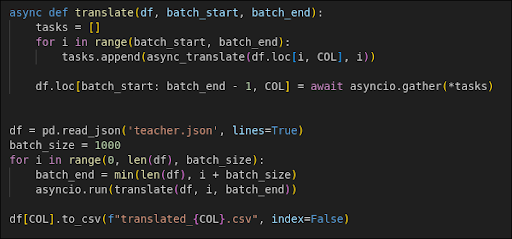
\includegraphics[width=0.75\linewidth]{figures/1.png}
\end{figure}
\newpage
Ngoài ra, chúng em nhận thấy không cần thiết phải dịch toàn bộ các trường dữ liệu lớn để huấn luyện mô hình vì một số trường dữ liệu không hỗ trợ cho việc huấn luyện mô hình. Thay vào đó, chúng em chỉ tập trung dịch 1 số trường sau đây:
\begin{quote}
-\textbf{course.json:} dịch cột “name”, “field”, “prerequisites” và “about”\\
\begin{figure}[h]
    \centering
    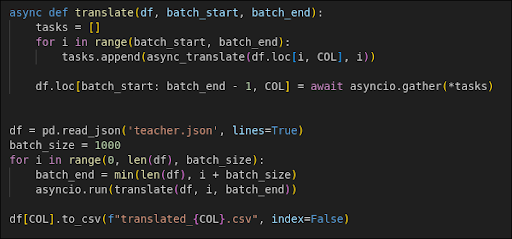
\includegraphics[width=1\linewidth]{figures/2.png}
\end{figure}\\
\\
\\
-\textbf{user.json:} dịch cột “school”\\
\begin{figure}[h]
    \centering
    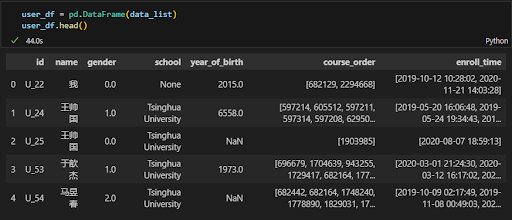
\includegraphics[width=0.8\linewidth]{figures/3.png}
\end{figure}
\newpage
-\textbf{teacher.json:} Tiến hành dịch tất cả (trừ “id” và “name”)\\
\begin{figure}[h]
    \centering
    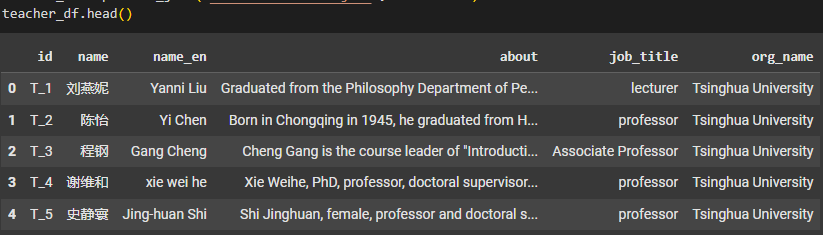
\includegraphics[width=1\linewidth]{figures/4.png}
\end{figure}\\
-\textbf{concept.json:} Dịch tất cả các cột của bảng này vì toàn bộ đều ở dạng chuỗi\\
\begin{figure}[h]
    \centering
    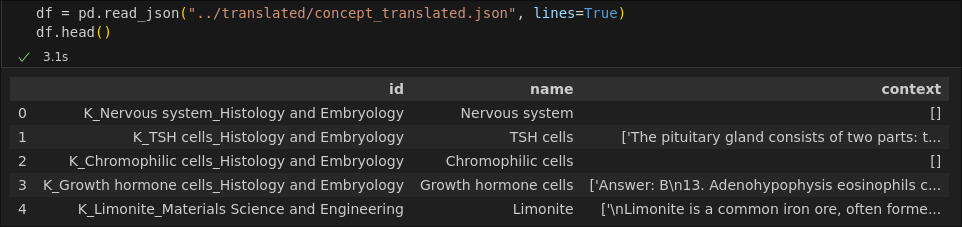
\includegraphics[width=1\linewidth]{figures/5.png}
\end{figure}\\
-\textbf{course-field.json:} Tiến hành dịch cột course\_name và field mang các thông tin dưới dạng chuỗi của bảng.\\
\begin{figure}[h]
    \centering
    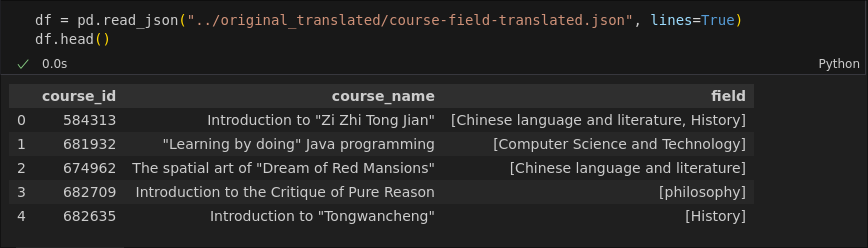
\includegraphics[width=1\linewidth]{figures/6.png}
\end{figure}
\end{quote}
\subsubsection{Khám phá dữ liệu}
\textbf{a) Bảng course.json}\\
Ta xem qua bảng course.json:
\begin{figure}[h]
    \centering
    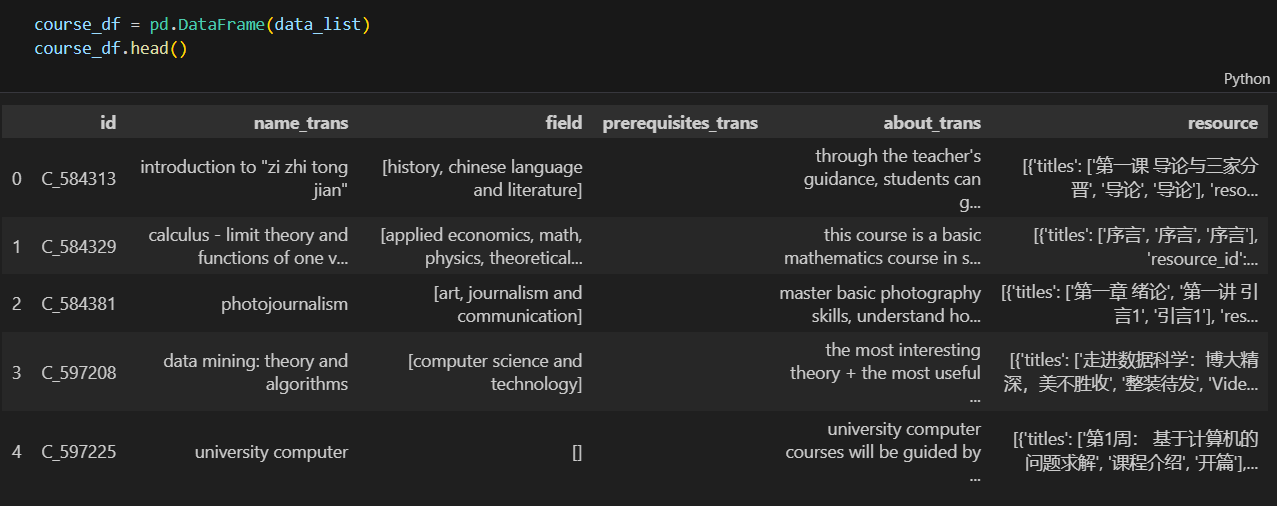
\includegraphics[width=1\linewidth]{figures/7.png}
\end{figure}\\
Ta xét độ dài của 3 cột “about”, “name\_trans” và “resource”:
\begin{figure}[h]
    \centering
    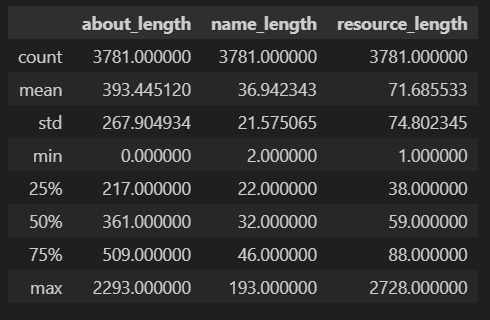
\includegraphics[width=0.485\linewidth]{figures/8.png}
\end{figure}
\newpage
Ta có thể thấy được 1 số thông tin từ dữ liệu trên:
\begin{itemize}
    \item Có những dòng dữ liệu không tồn tại cột “about”, tồn tại giá trị ngoại tệ ở cột “about” vì mean là 393 mà max lên đến 2293. Ta thể hiện trên boxplot độ dài của cột “about”:
    \begin{figure}[h]
        \centering
        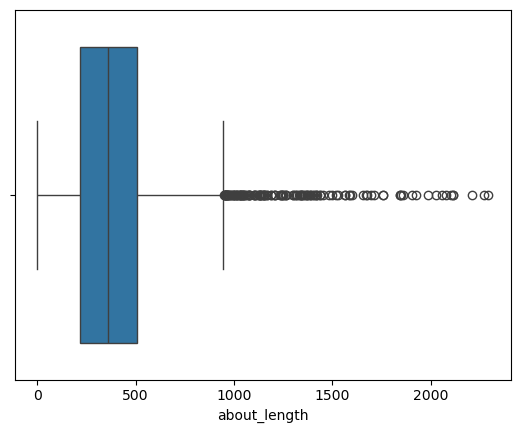
\includegraphics[width=0.75\linewidth]{figures/9.png}
    \end{figure}
    \item Có thể thấy thật sự nhiều giá trị ngoại tệ cần được xử lí.
    \item Có những dòng dữ liệu không có resource\_length, mean cũng rất ngắn (71) chứng tỏ ít thông tin về khoá học.
\end{itemize}
Ta phân tích sâu cột “resource”:
\begin{figure}[h]
    \centering
    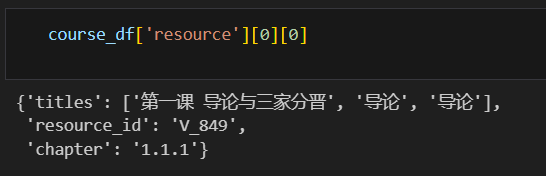
\includegraphics[width=0.75\linewidth]{figures/10.png}
\end{figure}\\
Mỗi resource trong bảng 2 là 1 tập hợp các video hay một tập các exercise. Mỗi resource sẽ có thêm 1 resource\_id là id của resource, chapter là chương chứa resource trong khóa học, titles gồm các tiêu đề như tiêu đề chương, video chương.\\
\\
Thông tin của resource có thể tìm thấy trong file course.json. Một resource có 2 loại: Video và Exercise. Nếu loại tài nguyên là video, nó được xác định bằng ID video bắt đầu bằng ký tự V\_. Nhiều video\_id khác nhau tương ứng với một ccid, và ccid xác định duy nhất một video. Các video\_id này tương ứng với việc hiển thị cùng một video ccid tại các thời gian bắt đầu khác nhau. Mối liên hệ giữa video\_id và ccid được lưu trong relations/video\_id-ccid.txt. Phụ đề video có thể được tìm thấy trong tệp entities/video.json thông qua ccid.\\
\\
Ta sẽ kiểm tra xem có bao nhiêu ID video không hợp lệ để phục vụ cho quá trình xử lý dữ liệu sau này:
\begin{figure}[h]
    \centering
    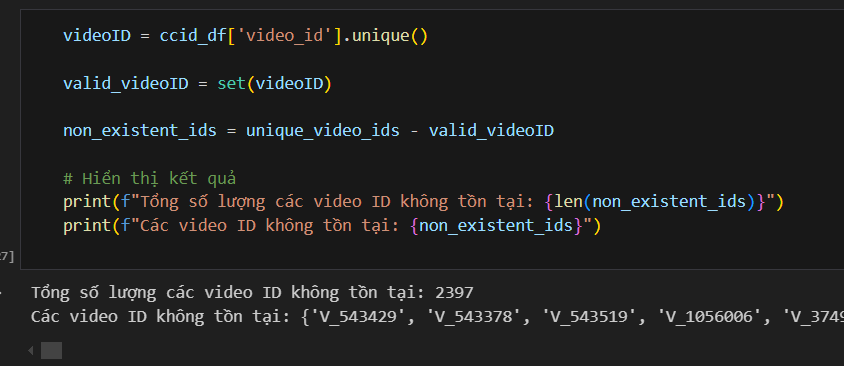
\includegraphics[width=0.75\linewidth]{figures/11.png}
\end{figure}\\
Có 2397 video ID không tồn tại, ta sẽ lọc đi hỗ trợ cho hiển thi thông tin trong tương lai.\\
\\
Ta bắt đầu tiến hành đếm số khoá học trong cột “name\_trans”, chia bởi lĩnh vực (cột “field”):\\
\begin{figure}[h]
    \centering
    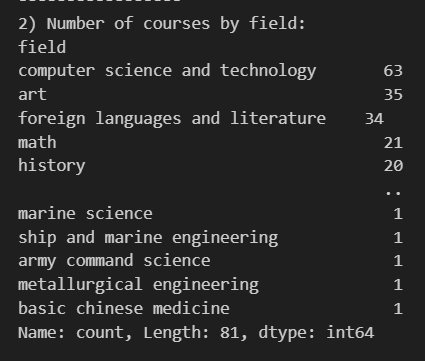
\includegraphics[width=0.35\linewidth]{figures/12.png}
\end{figure}
\newpage
\begin{figure}
    \centering
    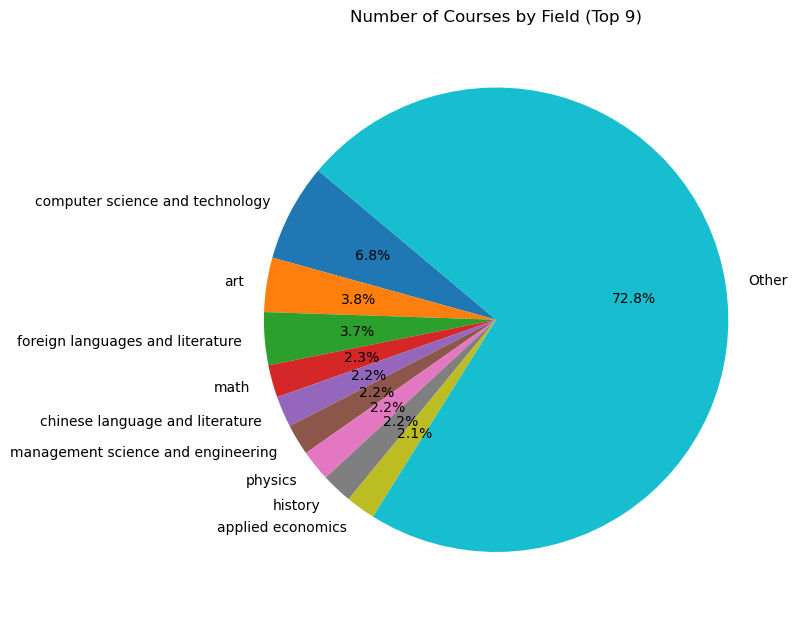
\includegraphics[width=0.7\linewidth]{figures/13.png}
\end{figure}
Ta thấy có tổng 3781 khoá học và 81 lĩnh vực, với “computer science and technology” đứng đầu với 63 khoá học, chiếm 6.8\% trên tổng khoá học. Ta cũng kiểm tra với mỗi khoá học được xếp bao nhiêu lĩnh vực (cột “field”):
\begin{figure}[h]
    \centering
    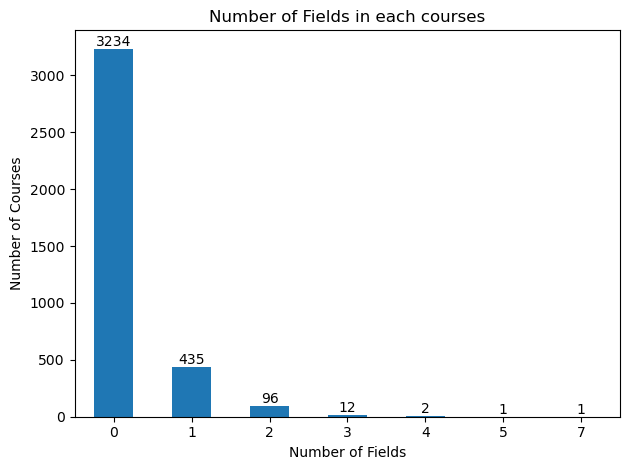
\includegraphics[width=0.9\linewidth]{figures/14.png}
\end{figure}\\
\newpage
Ta có thể thấy có rất nhiều khoá học không thuộc lĩnh vực nào, có rất nhiều khóa học không có field nào, có thể cột “field” sẽ không đóng góp nhiều trong xây dựng thuật toán hoặc cần xử lí.\\
\textbf{b) Bảng user.json}\\
Đầu tiên, ta đọc dữ liệu và quan sát dữ liệu thông qua dạng bảng (DataFrame):
\begin{figure}[h]
    \centering
    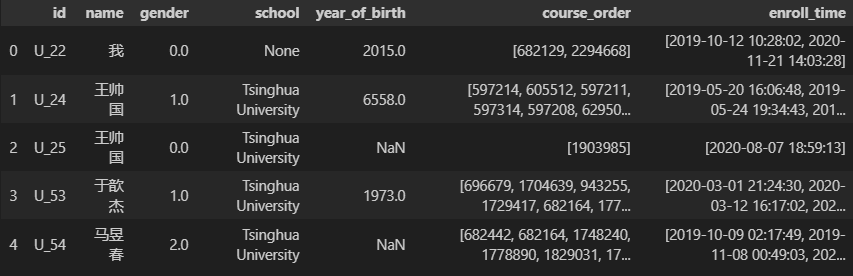
\includegraphics[width=1\linewidth]{figures/15.png}
\end{figure}
\newpage
Ta tiến hành thống kê đặc điểm từng cột có trong bảng:
\begin{figure}[h]
    \centering
    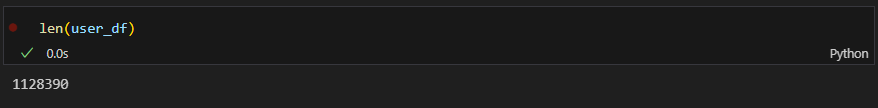
\includegraphics[width=1\linewidth]{figures/16.png}
    \caption{Số lượng users}
\end{figure}
\begin{figure}[h]
    \centering
    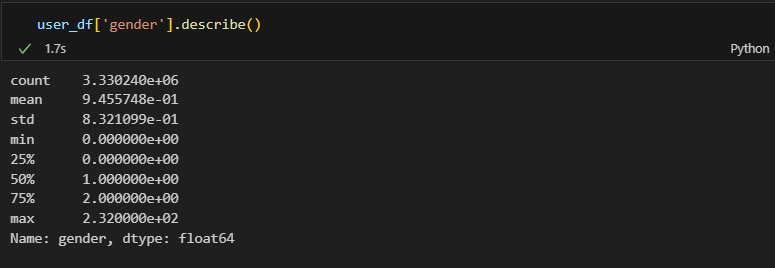
\includegraphics[width=1\linewidth]{figures/17.png}
    \caption{Cột “gender”}
\end{figure}
\begin{figure}[h]
    \centering
    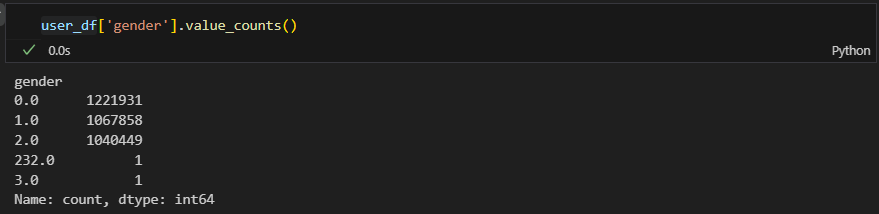
\includegraphics[width=1\linewidth]{figures/18.png}
    \caption{Phân bố các các giá trị trong cột “gender”:}
\end{figure}
\newpage
\begin{figure}
    \centering
    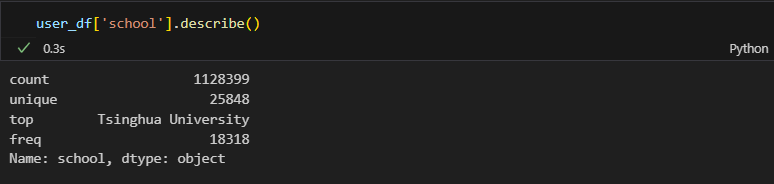
\includegraphics[width=1\linewidth]{figures/19.png}
    \caption{Thông tin cột “school”}
\end{figure}
\begin{figure}[h]
    \centering
    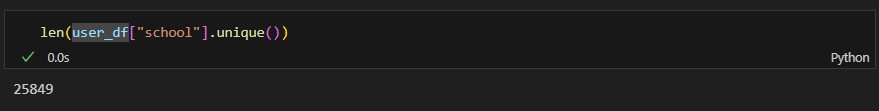
\includegraphics[width=1\linewidth]{figures/20.png}
    \caption{Số lượng trường học trong bảng}
\end{figure}
\begin{figure}[h]
    \centering
    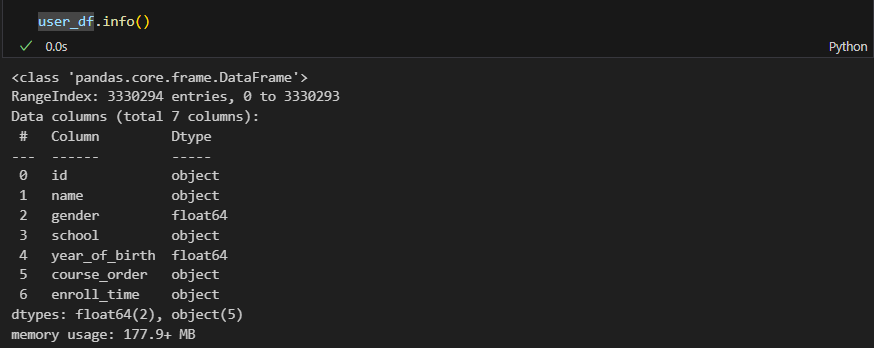
\includegraphics[width=1\linewidth]{figures/21.png}
    \caption{Kiểm tra thông tin tổng quan sau cùng}
\end{figure}
\newpage
\begin{figure}
    \centering
    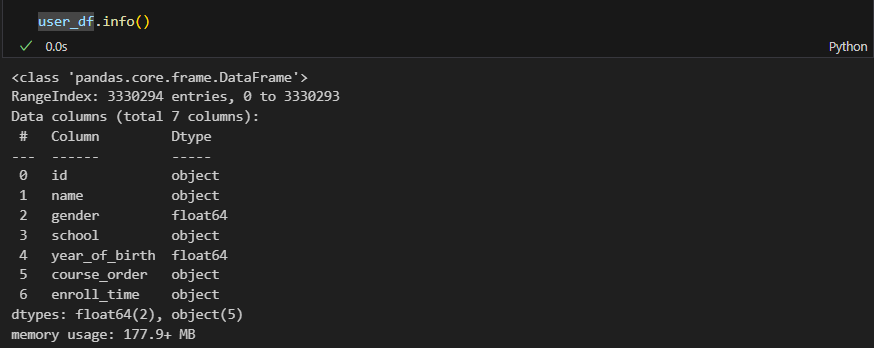
\includegraphics[width=1\linewidth]{figures/22.png}
    \caption{Số lượng sample (users) có trong bảng và số lượng users thuộc về mỗi trường học}
\end{figure}
\begin{figure}[h]
    \centering
    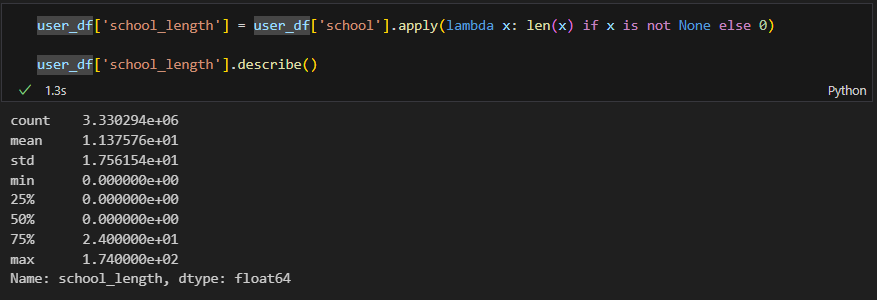
\includegraphics[width=1\linewidth]{figures/23.png}
    \caption{Tạo một cột “school\_length” để phân tích độ dài mỗi sample của cột}
\end{figure}
\newpage
\begin{figure}
    \centering
    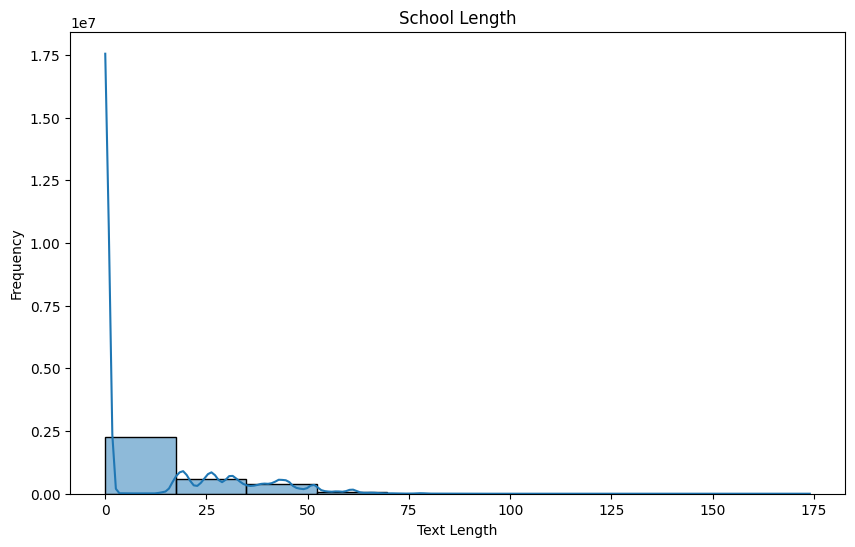
\includegraphics[width=0.68\linewidth]{figures/24.png}
    \caption{Trực quan hóa độ dài của sample cột “school”}
\end{figure}
\begin{figure}[h]
    \centering
    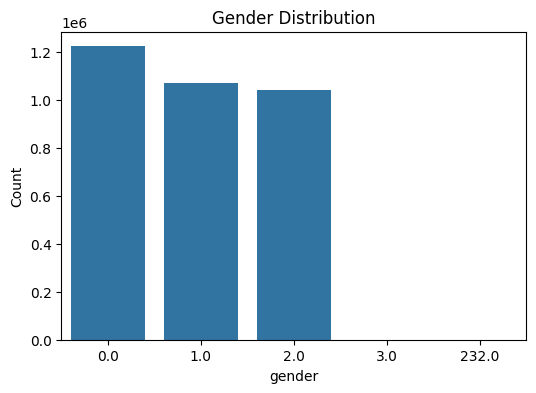
\includegraphics[width=0.68\linewidth]{figures/25.png}
    \caption{Trực quan hóa phân bố các giá trị của cột “gender”}
\end{figure}
\newpage
\textbf{c) Bảng teacher.json}\\
Sau đây là các thống số cơ bản của bảng
\begin{figure}[h]
    \centering
    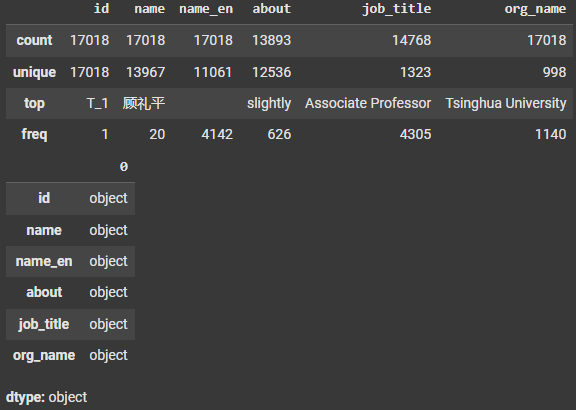
\includegraphics[width=0.6\linewidth]{figures/27.png}
\end{figure}\\
Tham khảo phân phối của top 10 tên việc xuất hiện nhiều nhất trong bảng
\begin{figure}[h]
    \centering
    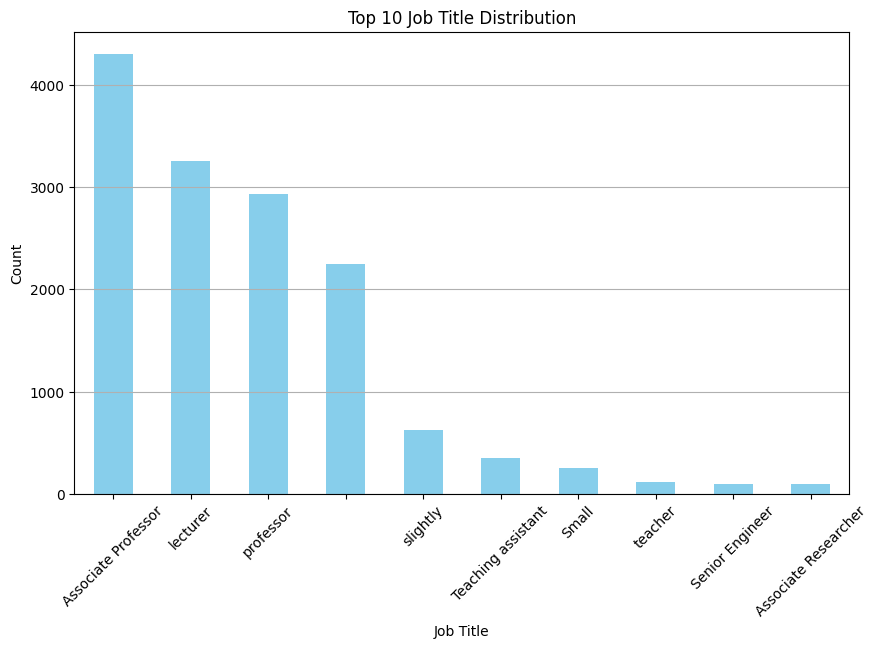
\includegraphics[width=0.75\linewidth]{figures/28.png}
\end{figure}\\
Tham khảo phân phối của top 10 tổ chức xuất hiện nhiều nhất trong bảng
\newpage
\begin{figure}
    \centering
    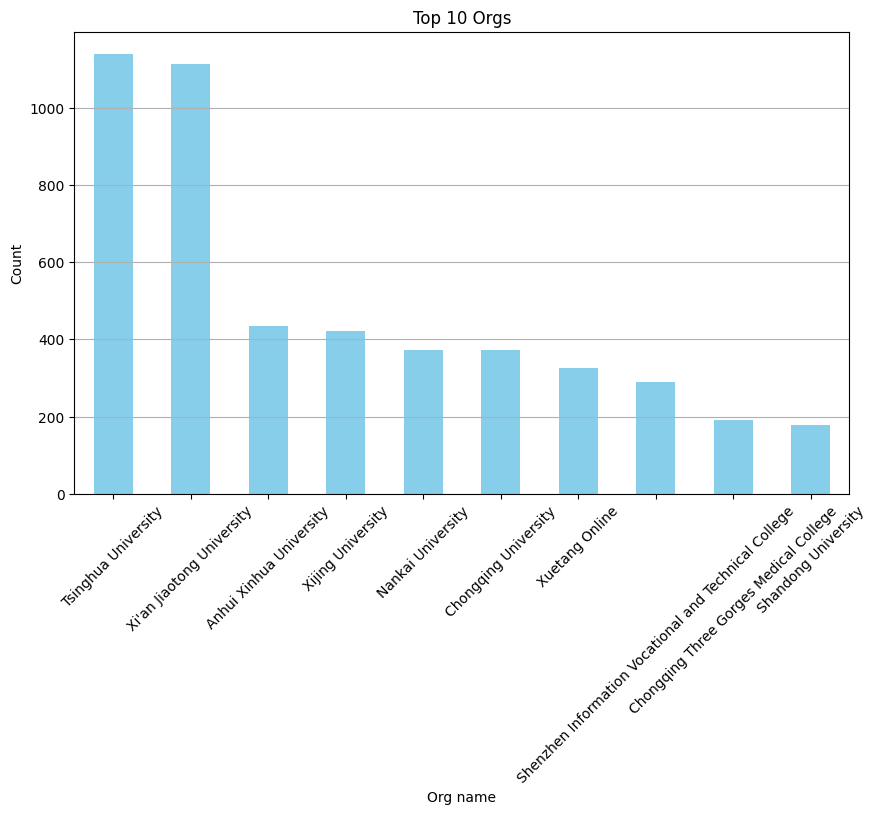
\includegraphics[width=0.75\linewidth]{figures/29.png}
\end{figure}
Ta thực hiện phân tích mối quan hệ giữa ba chức vụ (job titles) có số lượng giáo viên nhiều nhất và mười tổ chức (organizations) có số lượng giáo viên cao nhất
\begin{figure}[h]
    \centering
    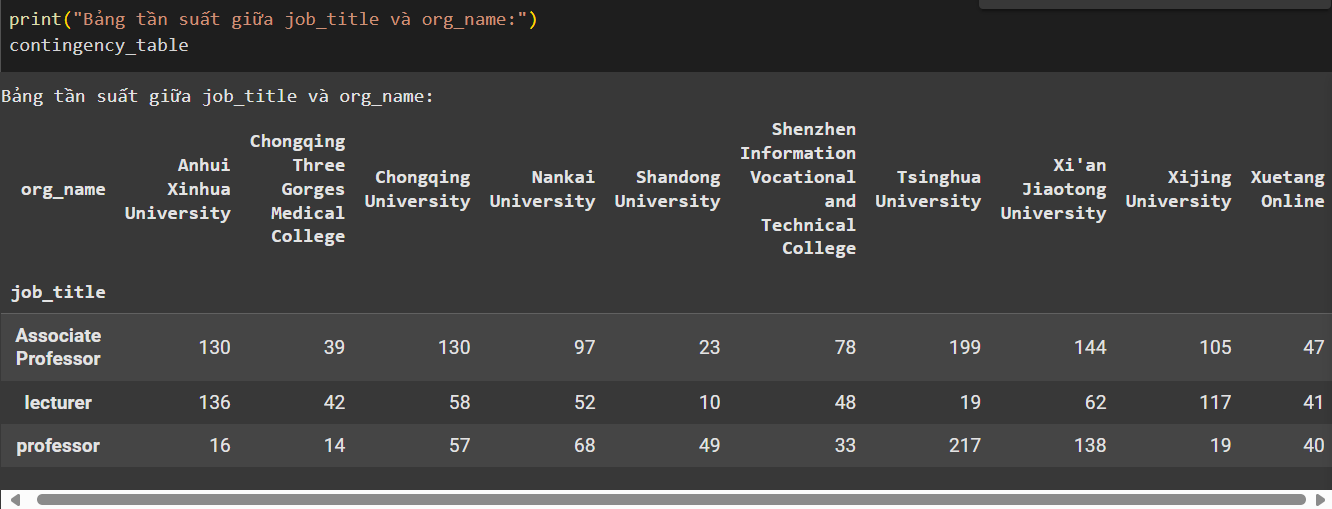
\includegraphics[width=0.95\linewidth]{figures/30.png}
\end{figure}
\newpage
\begin{figure}
    \centering
    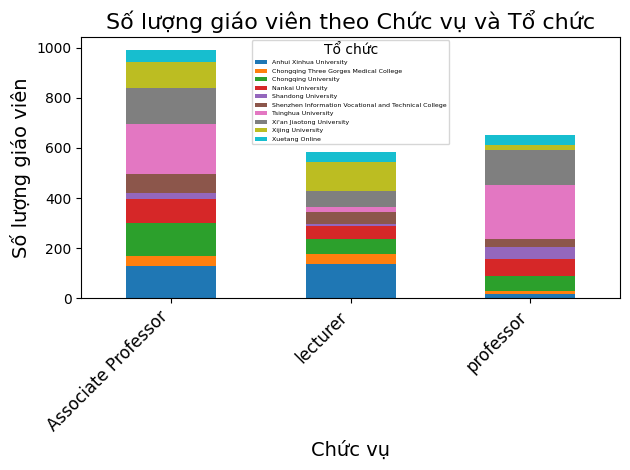
\includegraphics[width=0.65\linewidth]{figures/31.png}
\end{figure}
Sau khi lọc bỏ các liên kết có khóa học hoặc teacher không tồn tại dựa vào file course-teacher.txt, số hàng còn lại là 35593. Các thông tin được trực quan hóa như sau
\begin{figure}[h]
    \centering
    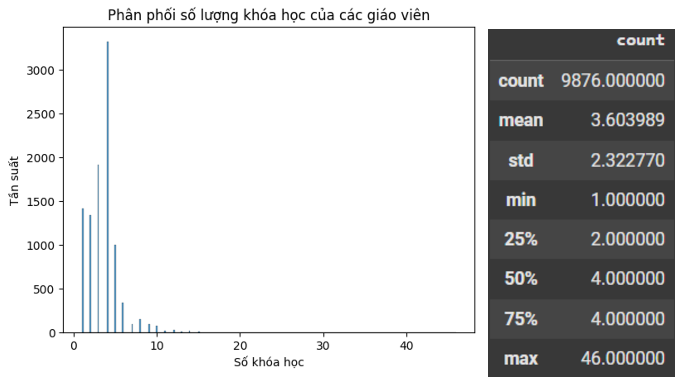
\includegraphics[width=0.8\linewidth]{figures/32.png}
    \caption{Histogram thể hiện số lượng khóa học của mỗi teacher và bảng thống kê mô tả tương ứng}
\end{figure}
\newpage
\begin{figure}
    \centering
    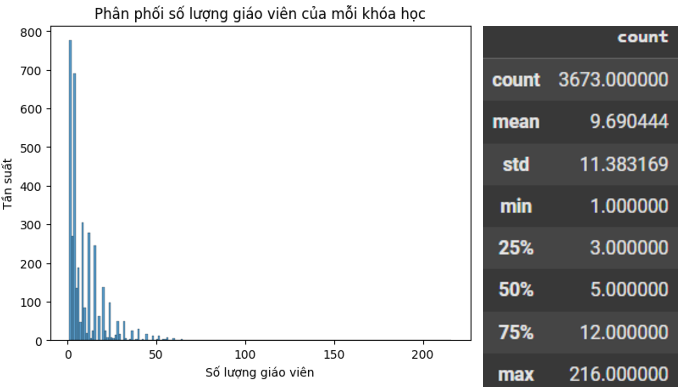
\includegraphics[width=0.8\linewidth]{figures/33.png}
    \caption{Histogram thể hiện số lượng teacher của mỗi khóa học và bảng thống kê mô tả tương ứng}
\end{figure}
\textbf{d) Bảng school.json}\\
Ta đếm dữ liệu ở từng cột, đếm các giá trị đặc biệt, giá trị xuất hiện nhiều nhất với tần số của nó:
\begin{figure}[h]
    \centering
    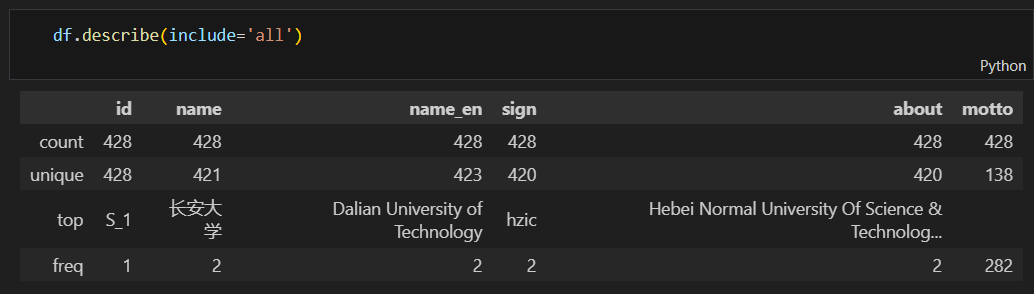
\includegraphics[width=0.75\linewidth]{figures/34.png}
\end{figure}\\
Kiểm tra kiểu dữ liệu của từng cột: 
\newpage
\begin{figure}
    \centering
    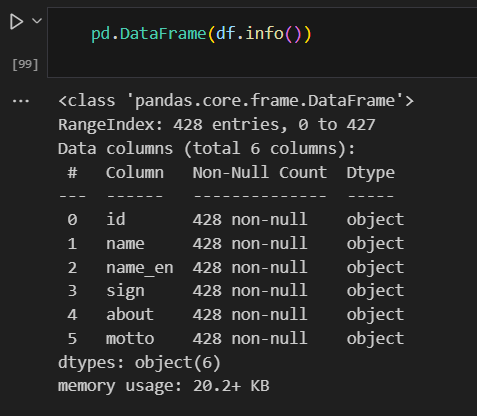
\includegraphics[width=0.6\linewidth]{figures/35.png}
\end{figure}
Ta tạo 2 cột mới là “about\_length” và “motto\_length” để lần lượt thể hiện độ dài của giá trị dữ liệu ở 2 cột “about” và “motto”:
\begin{figure}[h]
    \centering
    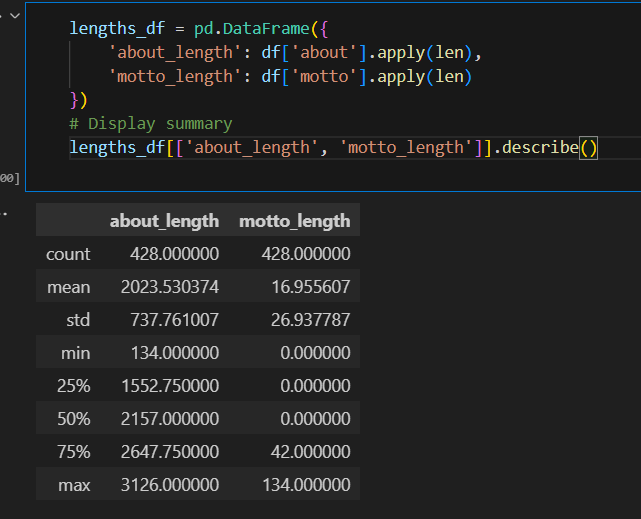
\includegraphics[width=0.65\linewidth]{figures/36.png}
\end{figure}
\newpage
Có 2 cột ta cần là “about\_length” và “motto\_length” để ta tìm phân bố độ dài của giá trị lên đồ thị:
\begin{figure}[h]
    \centering
    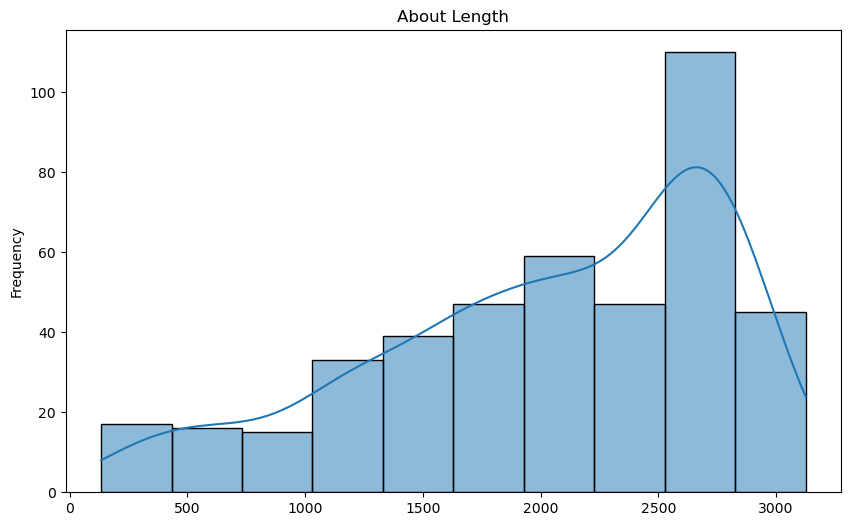
\includegraphics[width=0.7\linewidth]{figures/37.png}
\end{figure}\\
Dựa vào biểu đồ ta có thể nhận xét rằng mô tả của các trường đều rất chi tiết, số lượng trường với số lượng từ phần mô tả > 2000  chiếm phần lớn. Tuy nhiên thông tin này có vẻ không hữu ích với hệ thống khuyến nghị.
\begin{figure}[h]
    \centering
    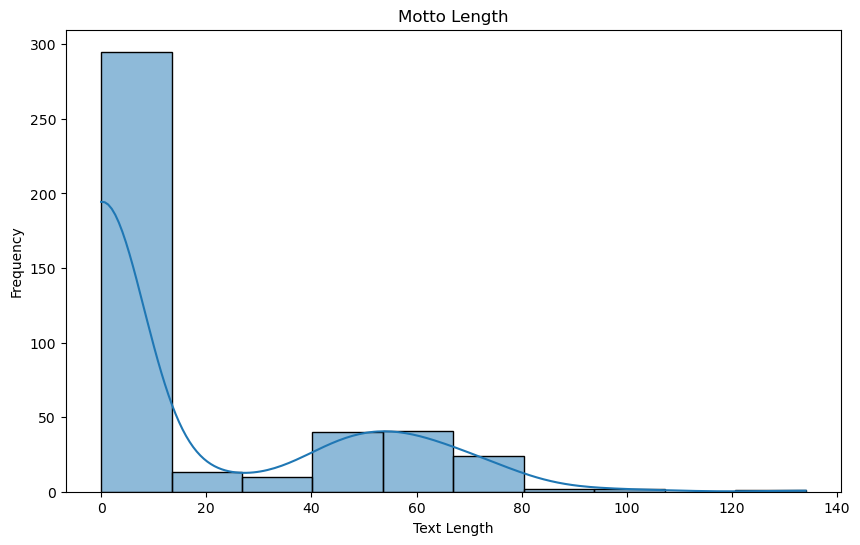
\includegraphics[width=0.7\linewidth]{figures/38.png}
\end{figure}\\
Hầu hết các trường đại học đều có một khẩu hiệu ngắn gọn dưới 20 từ vì chủ yếu khẩu hiệu sẽ đơn giản nhất có thể để truyền đạt tầm nhìn và mục tiêu của trường một cách trực tiếp ngắn gọn, đọng lại trong trí nhớ người xem. Một phần nhỏ hơn các trường có khẩu hiệu tương đối dài với 40 đến 88 chữ. 
\newpage
\textbf{e) Bảng course-field.json}
\begin{figure}[h]
    \centering
    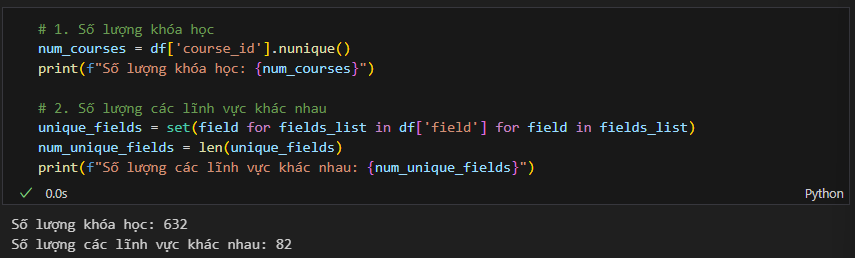
\includegraphics[width=1\linewidth]{figures/39.png}
    \caption{Tổng số lượng khóa học và tổng số lượng các lĩnh vực khác nhau}
\end{figure}
\begin{figure}[h]
    \centering
    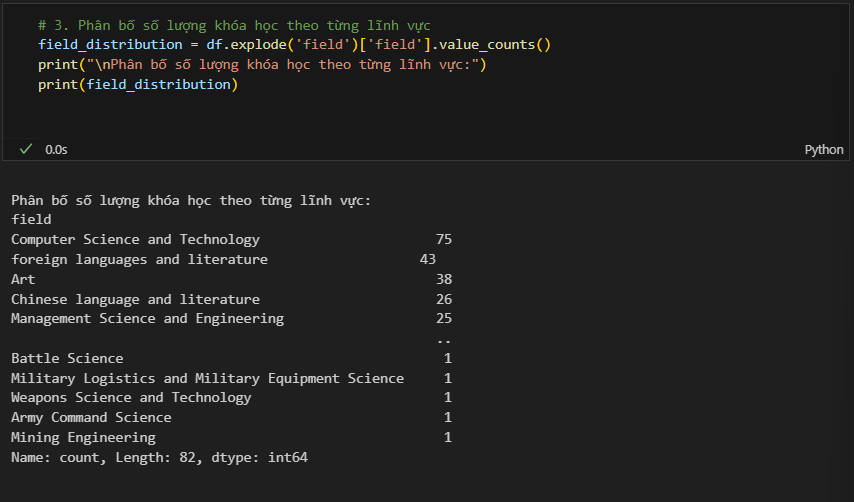
\includegraphics[width=1\linewidth]{figures/40.png}
    \caption{Phân bố số lượng khóa học theo từng lĩnh vực}
\end{figure}
\newpage
\begin{figure}
    \centering
    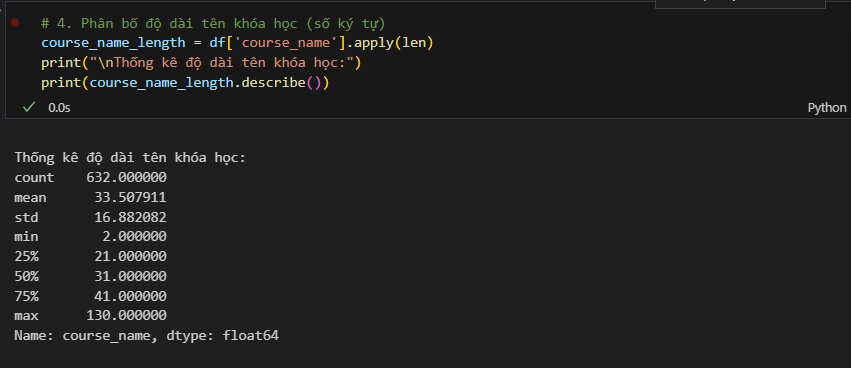
\includegraphics[width=0.85\linewidth]{figures/41.png}
    \caption{Phân bố độ dài tên khóa học}
\end{figure}
\begin{figure}[h]
    \centering
    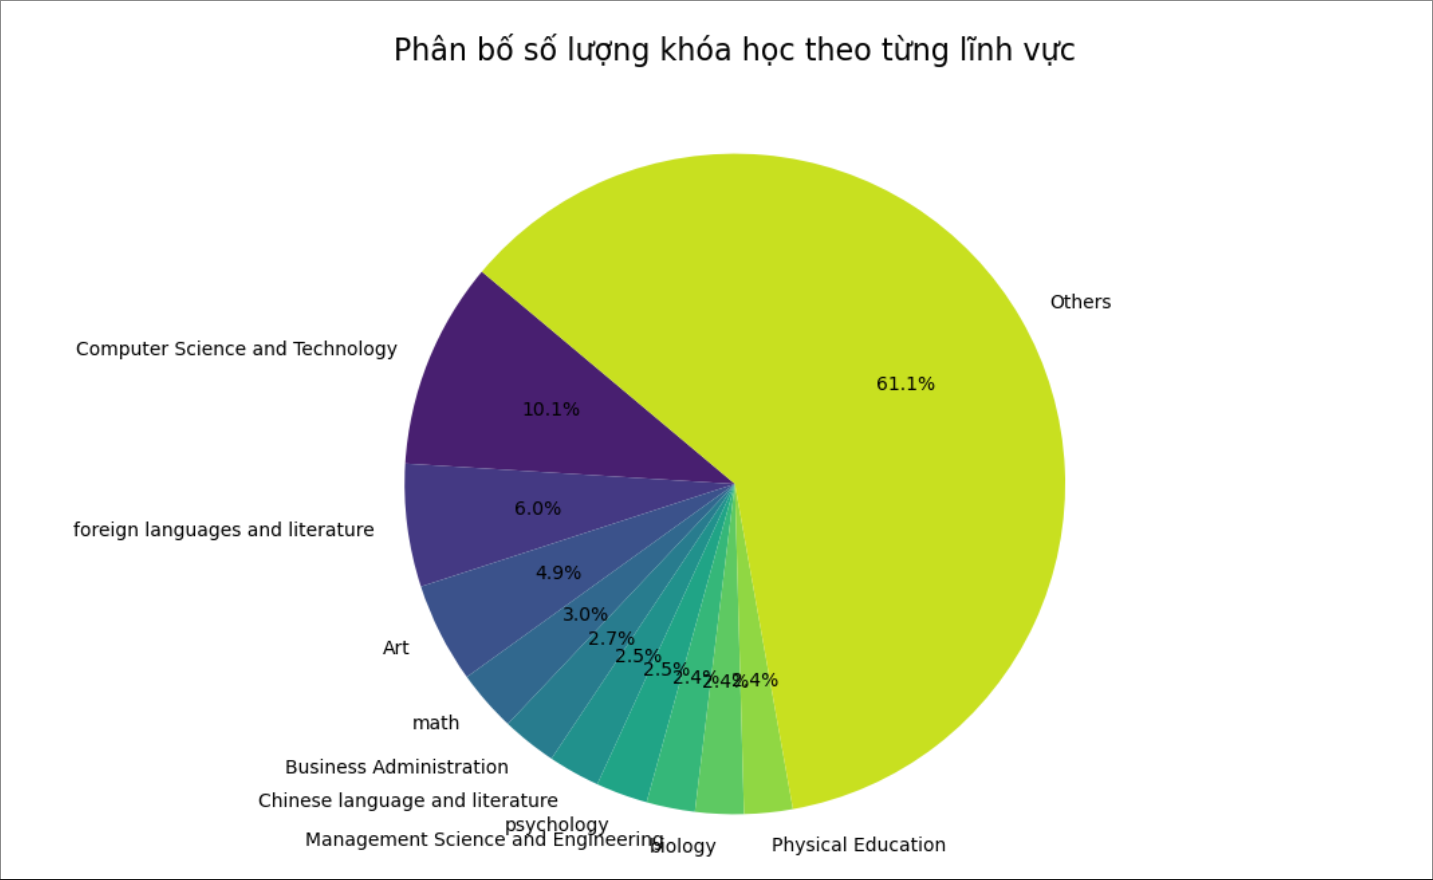
\includegraphics[width=0.9\linewidth]{figures/42.png}
    \caption{Biểu đồ thanh thể hiện sự phân bố số lượng khóa học theo từng lĩnh vực}
\end{figure}
\newpage
\begin{figure}
    \centering
    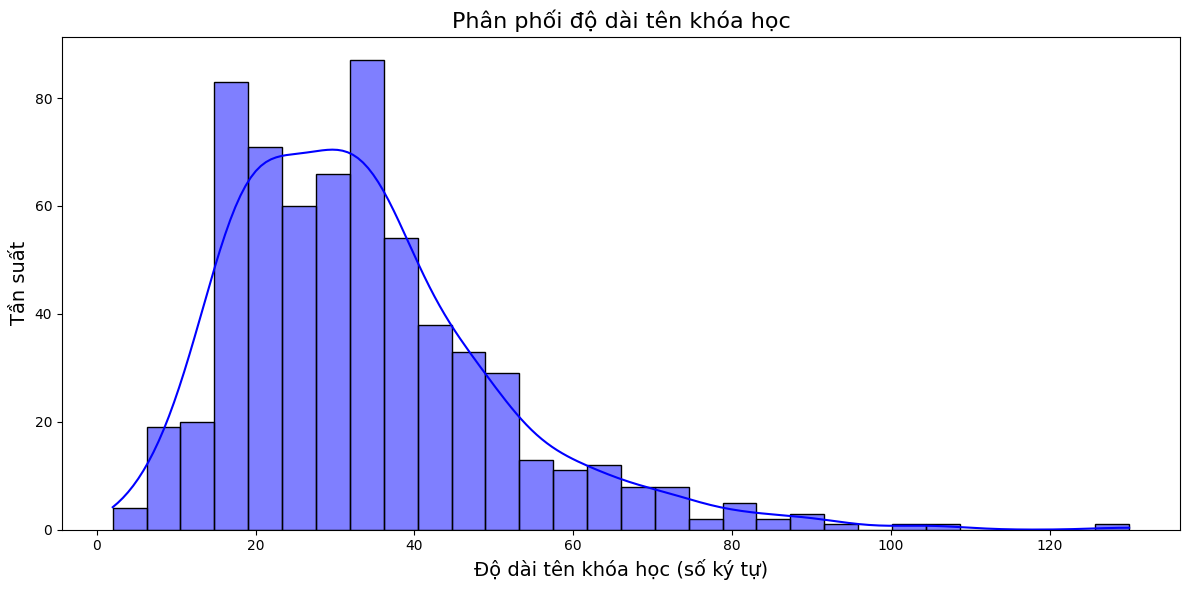
\includegraphics[width=0.75\linewidth]{figures/44.png}
    \caption{Biểu đồ phân phối cho độ dài tên khóa học}
\end{figure}
\subsubsection{Làm sạch dữ liệu}
\textbf{a) Bảng course.json}\\
Ta kiểm tra dữ liệu thiếu, dữ liệu không nhất quán, dữ liệu trùng lặp và dữ liệu trống:
\\
Đầu tiên ta thấy được có 647 giá trị ở cột “name\_trans” bị trùng lặp cho dù id không bị trùng, chứng tỏ có sự lỗi nhất định trong bộ dữ liệu, cũng như nãy đã thống kê ta thấy được có rất nhiều giá trị trống ở cột “field\_trans”.\\
\\
Ta kiểm tra kĩ hơn về các dòng có giá trị trong cột “name” bị trùng lặp:
\begin{figure}[h]
    \centering
    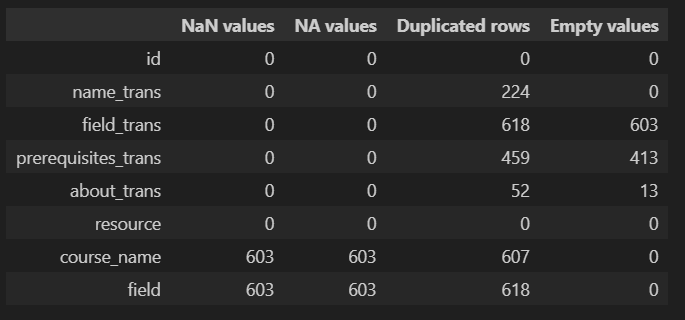
\includegraphics[width=1\linewidth]{figures/26.png}
\end{figure}
\newpage
\begin{figure}
    \centering
    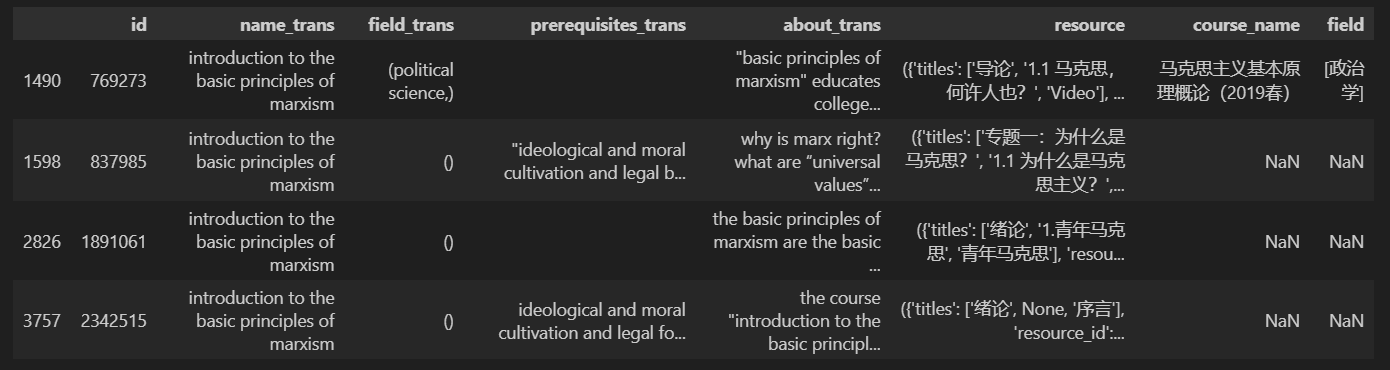
\includegraphics[width=1\linewidth]{figures/45.png}
\end{figure}
Ta thấy được đa số dữ liệu trong này cột “field” đa số bị trống và trùng lặp, cũng như các cột khác không có ý nghĩa hoặc trùng với các cột khác, thực hiện chi square test, ta có được kết quả với P-value rất thấp, chứng tỏ các giá trị phụ thuộc với nhau chứ không hề có giá trị mới. Chứng tỏ ta có thể xoá được các dòng dữ liệu này, cũng như các khoá học không tồn tại trong “course-field.json”.\\
\textbf{b) Bảng user.json}\\
Ta thấy cột “year\_of\_birth” bị thiếu dữ liệu hơn 97\% trong khi các cột còn lại tỉ lệ \% thiếu là rất thấp. Ta tiến hành loại bỏ cột này, sau đó ta sẽ tiến hành xử lý dữ liệu nhiễu trên cột gender với 2 giá trị nhiễu là 232 và 3\\
\textbf{c) Bảng concept.json}\\
Xử lý dữ liệu thiếu giúp cải thiện độ chính xác của mô hình, đảm bảo tính toàn vẹn của phân tích, tránh lỗi tính toán và giảm độ thiên lệch. Một số cách xử lý phổ biến gồm:\\
\begin{itemize}
    \item Loại bỏ hàng/cột: Áp dụng khi dữ liệu thiếu quá nhiều.
    \item Điền giá trị thay thế: Điền trung bình, trung vị, hoặc giá trị dự đoán vào chỗ thiếu.
    \item Dùng mô hình dự đoán: Áp dụng các thuật toán để dự đoán giá trị thiếu.
\end{itemize}
Việc xử lý phù hợp giúp dữ liệu chính xác và đáng tin cậy hơn trong phân tích và dự đoán.\\
\newpage
\begin{figure}
    \centering
    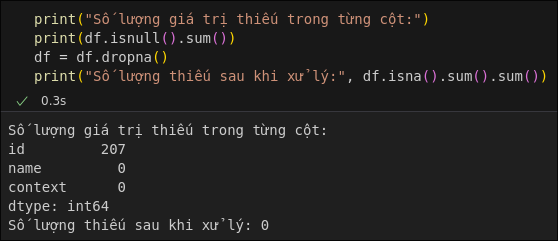
\includegraphics[width=1\linewidth]{figures/46.png}
\end{figure}
Xử lý dữ liệu trùng lặp là bước quan trọng trong tiền xử lý dữ liệu nhằm loại bỏ các bản ghi trùng lặp để đảm bảo tính chính xác và hiệu quả của mô hình. Dữ liệu trùng lặp có thể gây sai lệch và làm chậm quá trình xử lý.\\
Các phương pháp xử lý dữ liệu trùng lặp phổ biến bao gồm:\\
\begin{itemize}
    \item Xóa các bản ghi trùng lặp: Loại bỏ các hàng hoàn toàn trùng lặp trong DataFrame bằng hàm drop\_duplicates() trong Pandas.
    \item Giữ lại bản ghi đầu tiên hoặc cuối cùng: Nếu cần giữ lại một bản ghi đại diện, có thể chỉ xóa các bản trùng lặp sau hoặc trước.
    \item Xác định tiêu chí trùng lặp: Tìm và xóa bản ghi trùng lặp dựa trên một số cột cụ thể thay vì toàn bộ hàng.
\end{itemize}
Loại bỏ dữ liệu trùng lặp giúp dữ liệu trở nên nhất quán, giảm dung lượng và cải thiện độ chính xác của phân tích và mô hình.\\
Loại bỏ dữ liệu với phương thức drop\_duplicates():
\newpage
\begin{figure}
    \centering
    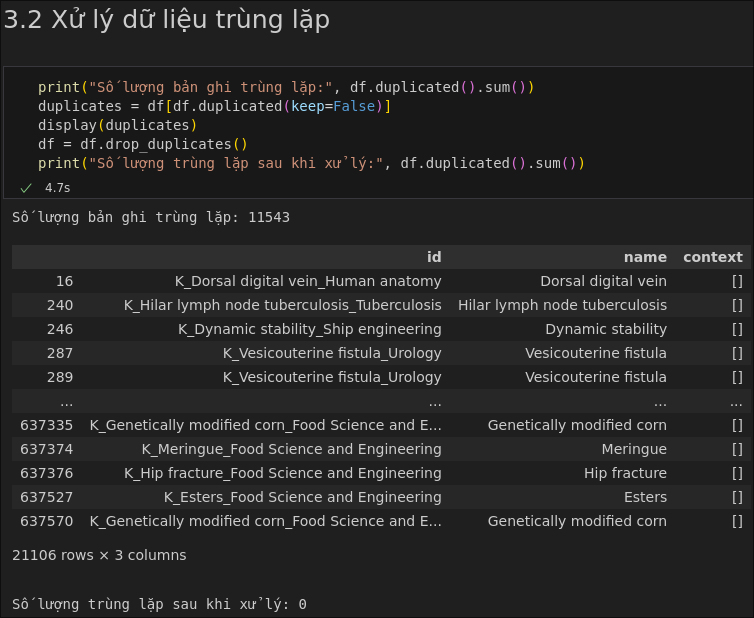
\includegraphics[width=1\linewidth]{figures/47.png}
\end{figure}
\textbf{d) Bảng course-field.json}\\
Sử dụng isnull().sum() để tính số lượng giá trị thiếu trong từng cột. Sau đó loại bỏ hàng chứa giá trị thiếu bằng cách sử dụng dropna()
\newpage
\begin{figure}
    \centering
    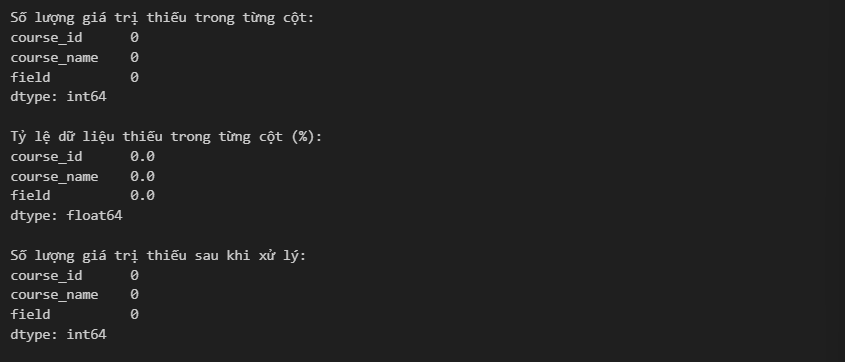
\includegraphics[width=1\linewidth]{figures/48.png}
\end{figure}
Dữ liệu văn bản thường chứa nhiều thông tin nhiễu chẳng hạn như các ký tự không mong muốn: Các ký tự đặc biệt, dấu câu, hoặc ký tự không phải chữ cái có thể làm giảm chất lượng phân tích. Ở đây chúng ta sẽ tiến hành loại bỏ các ký tự không cần thiết, các khoảng trắng dư thừa và thường hóa các ký tự viết hoa\\
\\
Để kiếm tra dữ liệu trùng lặp, chúng ta sử dụng phương thức duplicated() trong pandas. Đầu tiên xác định các bản ghi trùng lặp, sau đó đếm số lượng và hiển thị các bảng ghi trùng lặp đó. Sau đó tiến hành xóa bản ghi trùng lặp bằng cách sử dụng drop\_duplicates()
\newpage
\begin{figure}
    \centering
    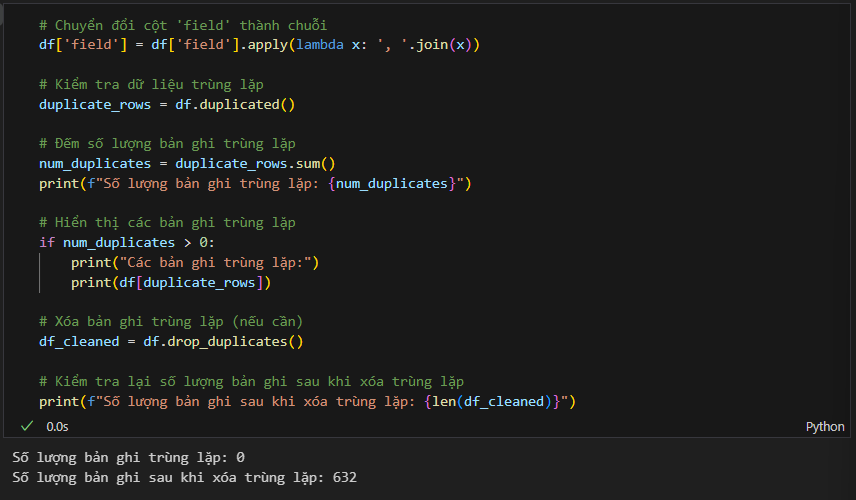
\includegraphics[width=1\linewidth]{figures/49.png}
\end{figure}
\textbf{e) Bảng school.json}\\
Ta xoá cột “name” đi vì trùng với ý nghĩa với cột “name\_en” (tên nhưng trong Tiếng Anh)\\
\\
Ta thống nhất cột “sign” (kí hiệu đại diện cho trường) đều là tất cả in hoa:
\newpage
\begin{figure}
    \centering
    \includegraphics[width=0.7\linewidth]{figures/50.png}
\end{figure}
Vì ở đây tên trường (“name\_en”) cũng như kí hiệu (“sign”) là chìa khoá chính, hay nói cách khác là giá trị duy nhất nên không thể có dòng trùng với nhau, ta tiến hành xoá các dòng trùng giá trị:
\begin{figure}[h]
    \centering
    \includegraphics[width=0.7\linewidth]{figures/51.png}
\end{figure}\\
\textbf{g) Bảng teacher.json}\\
Ở đây có cột name\_en bị thiếu nên điền vào cột đó bằng cách lấy phiên âm của cột name là được. Để làm việc này có thể sử dụng thư viện pypinyin để lấy phát âm dùng cho tên tiếng anh.
\newpage
\begin{figure}
    \centering
    \includegraphics[width=0.8\linewidth]{figures/52.png}
\end{figure}
\subsubsection{Chuyển đổi dữ liệu}
\textbf{Feature Engineering:}
Nhóm sẽ chọn các bảng và thuộc tính có thể sử dụng để tạo ra feature các mô hình khuyến nghị dựa trên bộ dữ liệu đã xử lý và làm sạch trước đó:\\
\\
Các bảng được chọn và thuộc tính sử dụng:
\begin{figure}[h]
    \centering
    \includegraphics[width=0.6\linewidth]{figures/53.png}
\end{figure}
\newpage
\begin{itemize}
    \item Với ‘user.json’: ‘course\_order’ gồm các khóa học mà user đã đăng ký với khóa học sau cùng là khóa học gần đây nhất, dùng để tạo liên kết giữa ‘user.json’ và ‘course.json’.
    \item Với ‘course.json’: Đây là table quan trọng chứa thông tin về các khóa học như ‘name’, ‘about’ và ‘field’.
    \item Với ‘teacher.json’, ‘school.json’: dùng để tạo relation với ‘course.json’ chứa thông tin về trường tổ chức khóa học và giáo viên giảng dạy.
    \item Với ‘course-field.json’: chứa các field của mỗi khóa học, dùng để kiểm tra với trường ‘field’ trong ‘course.json’.
    \item Với ‘concept.json’: id theo quy ước ‘K\_{concept name}{field}’, tạo thêm feature concept-name\_field với mỗi khoá học.
\end{itemize}
Tạo knowledge graph:
\begin{figure}[h]
    \centering
    \includegraphics[width=0.3\linewidth]{figures/54.png}
\end{figure}\\
Tạo interaction giữa người dùng với khóa học: sử dụng 5-core filtering, lọc người dùng với ít hơn 5 khóa học và những khóa học có số lượng đăng ký dưới 5.\\
\\
Kết quả: Vì data đã được xử lý trước đó nên ta thấy không có thay đổi đáng kể
\begin{center}
\begin{tabular}{|| m{15em}  m{15em}||} 
 \hline
 Trước khi filter & Sau khi filter\\ [0.5ex] 
 \hline\hline
 1.183.774 interactions & 1.182.745 interactions \\ [1ex]
 \hline
\end{tabular}
\end{center}
\newpage
Tạo relation giữa các entities: course-relation-attribute. Sau đó ta tiến hành lọc theo tiêu chí, số lần course xuất hiện tối thiểu là 5 và số lần xuất hiện tối thiểu của một relation là 25. \\
\\
Kết quả: 
\begin{center}
\begin{tabular}{|| m{15em}  m{15em}||} 
 \hline
 Trước khi filter & Sau khi filter\\ [0.5ex] 
 \hline\hline
 376.093 interactions & 71.787 interactions \\ [1ex]
 \hline
\end{tabular}
\end{center}
\subsection{Phân tích vấn đề}
Hệ thống học tập trực tuyến MOOC cung cấp số lượng lớn các khóa học đa dạng, nhưng khó khăn lớn đối với người học là tìm kiếm khóa học phù hợp với sở thích và nhu cầu cá nhân. Để giải quyết vấn đề này, hệ thống khuyến nghị khóa học được phát triển nhằm cá nhân hóa trải nghiệm học tập cho từng người dùng dựa trên dữ liệu về hành vi học tập và các đặc điểm cá nhân.\\
\\
Bài toán đặt ra trong dự án này là: \textbf{Làm thế nào để xây dựng một hệ thống khuyến nghị khóa học cá nhân hóa cho từng người học trên nền tảng MOOC?}
\subsubsection{Câu hỏi nghiên cứu}
\begin{itemize}
    \item Làm thế nào để dự đoán chính xác các khóa học mà một người dùng có khả năng sẽ đăng ký tiếp theo?
    \item Làm sao tận dụng các đặc điểm của người dùng như giới tính, độ tuổi, trường học, và lịch sử khóa học để tăng độ chính xác của mô hình khuyến nghị?
    \item Làm sao đánh giá chất lượng các gợi ý khóa học và xác định mức độ hiệu quả của hệ thống (metric đánh giá là gì) ?
\end{itemize}
\subsubsection{Kết quả đề tài}
Dự án hướng tới xây dựng một hệ thống khuyến nghị khóa học hiệu quả, dựa trên dữ liệu của người học từ bộ MOOCCubeX. Kết quả mong muốn bao gồm:
\begin{itemize}
    \item \textbf{Xác định yếu tố ảnh hưởng đến việc đăng ký khóa học:} Khám phá các đặc điểm người dùng (giới tính, trường học, năm sinh, các khóa học đã đăng ký...) ảnh hưởng đến hành vi chọn khóa học. Điều này giúp hệ thống có cái nhìn rõ ràng hơn về các yếu tố quan trọng khi gợi ý khóa học.
    \item \textbf{Khả năng khuyến nghị khóa học cá nhân hóa:} Kỳ vọng hệ thống sẽ đưa ra những gợi ý chính xác cho từng người học, dựa trên hành vi đăng ký khóa học trước đây và các yếu tố liên quan. Mục tiêu là hệ thống có thể dự đoán tốt các khóa học mà người dùng có khả năng quan tâm trong tương lai.
    \item \textbf{Định hướng cải thiện trải nghiệm học tập:} Hệ thống khuyến nghị dự kiến sẽ giúp người học tiết kiệm thời gian tìm kiếm, đồng thời cung cấp cho họ trải nghiệm học tập tốt hơn thông qua việc gợi ý các khóa học phù hợp với mục tiêu và sở thích cá nhân.
    \item \textbf{Đánh giá các phương pháp tiếp cận:} Tìm hiểu các mô hình Recommendation System và thử nghiệm với bộ dữ liệu để so sánh độ hiệu quả của các mô hình.
\end{itemize}
\subsection{Khả năng ứng dụng}
Hệ thống khuyến nghị này có tiềm năng ứng dụng rộng rãi trong các nền tảng học tập trực tuyến. Cụ thể:
\begin{itemize}
    \item \textbf{Cá nhân hóa trải nghiệm học tập:} Giúp người dùng nhanh chóng tìm được các khóa học phù hợp với mục tiêu học tập và sở thích cá nhân. Tăng cường trải nghiệm người dùng.
    \item \textbf{Thu hút người dùng:} Các gợi ý chính xác và kịp thời có thể dẫn đến tỷ lệ đăng ký khóa học cần thiết cao hơn và cải thiện sự gắn bó của người dùng với nền tảng. Các khóa học phù hợp và hấp dẫn có thể giúp giảm tỷ lệ người học từ bỏ giữa chừng, cải thiện tỷ lệ hoàn thành khóa học.
    \item \textbf{Nâng cao hiệu suất học tập của người dùng:} Từ những hành vi học tập của người dùng trong quá khứ, hệ thống sẽ căn cứ vào và tự động đề xuất các khóa học tương thích nhất với khả năng và kỹ năng của người học để tối ưu hóa nhất hiệu suất học tập của người dùng.
\end{itemize}



\newpage



% ----------------------------------------------------------------------------------------
\end{document}
